\documentclass{article}
\usepackage[utf8]{inputenc}
\usepackage{url}
\usepackage{amsmath, amsthm, amssymb, amsfonts}
\usepackage{amssymb}
\usepackage{tikz}
\usepackage{rubikcube,rubikrotation,rubikpatterns,rubiktwocube}
\usepackage{color}
\usepackage{floatrow}
\usepackage{listings}
%\usepackage{minted}
\usepackage{fancyhdr}
\pagestyle{fancy}
\fancyhf{}
\fancyhead[R]{\thepage}
\usepackage{biblatex}
\addbibresource{bibliography.bib}
%\usepackage{apacite}
\lstset{ %
language=C++,                % choose the language of the code
basicstyle=\footnotesize,       % the size of the fonts that are used for the code
numbers=left,                   % where to put the line-numbers
numberstyle=\footnotesize,      % the size of the fonts that are used for the line-numbers
stepnumber=1,                   % the step between two line-numbers. If it is 1 each line will be numbered
numbersep=5pt,                  % how far the line-numbers are from the code
backgroundcolor=\color{white},  % choose the background color. You must add \usepackage{color}
showspaces=false,               % show spaces adding particular underscores
showstringspaces=false,         % underline spaces within strings
showtabs=false,                 % show tabs within strings adding particular underscores
frame=single,           % adds a frame around the code
tabsize=2,          % sets default tabsize to 2 spaces
captionpos=b,           % sets the caption-position to bottom
breaklines=true,        % sets automatic line breaking
breakatwhitespace=false,    % sets if automatic breaks should only happen at whitespace
escapeinside={\%*}{*)}          % if you want to add a comment within your code
}

\usepackage{caption}

\markright{\textsc{rubikcube} package; \hspace{2cm}file = main.tex}
%% increase textwidth to make room 
\addtolength{\oddsidemargin}{-1.5cm}
\addtolength{\textwidth}{3cm}
%% brace and bracket 
\newcommand{\Rubikbracket}[1]{$\left(\mbox{#1}\right)$}
\newcommand{\Rubikbrace}[1]{$\left\{\mbox{#1}\right\}$}
\author{Ellis Pridgeon}
\title{The Mathematics of the Rubik's Cube}\vspace{-50pt}
\date{Date of Hand in: June 1st 2018}

\usepackage{physics}
\usepackage{mathtools}
\DeclarePairedDelimiter{\opair}{\langle}{\rangle}
\newtheorem{theorem}{Theorem}[section]
\newtheorem{lemma}[section]{Lemma}
\newtheorem{proposition}[section]{Proposition}
\usepackage{afterpage}

\usepackage{tcolorbox}
\tcbuselibrary{theorems}

\newtcbtheorem[number within=section]{myinput}{Input}%
{colback=green!5,colframe=green!35!black,fonttitle=\bfseries}{ip}

\newtcbtheorem[number within=section]{myoutput}{Output}%
{colback=green!5,colframe=red!35!black,fonttitle=\bfseries}{op}

\usepackage[framemethod=TikZ]{mdframed}
%-------------------------------------------------------
\newcounter{theo}[section]\setcounter{theo}{0}
\renewcommand{\thetheo}{\arabic{section}.\arabic{theo}}
\newenvironment{theo}[2][]{%
\refstepcounter{theo}%
\ifstrempty{#1}%
{\mdfsetup{%
frametitle={%
\tikz[baseline=(current bounding box.east),outer sep=0pt]
\node[anchor=east,rectangle,fill=blue!20]
{\strut Theorem~\thetheo};}}
}%
{\mdfsetup{%
frametitle={%
\tikz[baseline=(current bounding box.east),outer sep=0pt]
\node[anchor=east,rectangle,fill=blue!20]
{\strut Theorem~\thetheo:~#1};}}%
}%
\mdfsetup{innertopmargin=10pt,linecolor=blue!20,%
linewidth=2pt,topline=true,%
frametitleaboveskip=\dimexpr-\ht\strutbox\relax
}
\begin{mdframed}[]\relax%
\label{#2}}{\end{mdframed}}
%-------------------------------------------------------
\newcounter{defn}[section]\setcounter{defn}{0}
\renewcommand{\thedefn}{\arabic{section}.\arabic{defn}}
\newenvironment{defn}[2][]{%
\refstepcounter{defn}%
\ifstrempty{#1}%
{\mdfsetup{%
frametitle={%
\tikz[baseline=(current bounding box.east),outer sep=0pt]
\node[anchor=east,rectangle,fill=brown!20]
{\strut Definition~\thedefn};}}
}%
{\mdfsetup{%
frametitle={%
\tikz[baseline=(current bounding box.east),outer sep=0pt]
\node[anchor=east,rectangle,fill=brown!20]
{\strut Definition~\thedefn:~#1};}}%
}%
\mdfsetup{innertopmargin=10pt,linecolor=brown!20,%
linewidth=2pt,topline=true,%
frametitleaboveskip=\dimexpr-\ht\strutbox\relax
}
\begin{mdframed}[]\relax%
\label{#2}}{\end{mdframed}}
%-------------------------------------------------------
\newcounter{prop}[section]\setcounter{prop}{0}
\renewcommand{\theprop}{\arabic{section}.\arabic{prop}}
\newenvironment{prop}[2][]{%
\refstepcounter{prop}%
\ifstrempty{#1}%
{\mdfsetup{%
frametitle={%
\tikz[baseline=(current bounding box.east),outer sep=0pt]
\node[anchor=east,rectangle,fill=yellow!20]
{\strut Proposition~\theprop};}}
}%
{\mdfsetup{%
frametitle={%
\tikz[baseline=(current bounding box.east),outer sep=0pt]
\node[anchor=east,rectangle,fill=yellow!20]
{\strut Proposition~\theprop:~#1};}}%
}%
\mdfsetup{innertopmargin=10pt,linecolor=yellow!20,%
linewidth=2pt,topline=true,%
frametitleaboveskip=\dimexpr-\ht\strutbox\relax
}
\begin{mdframed}[]\relax%
\label{#2}}{\end{mdframed}}

%---------------------------------------------------
\newcounter{lem}[section]\setcounter{lem}{0}
\renewcommand{\thelem}{\arabic{section}.\arabic{lem}}
\newenvironment{lem}[2][]{%
\refstepcounter{lem}%
\ifstrempty{#1}%
{\mdfsetup{%
frametitle={%
\tikz[baseline=(current bounding box.east),outer sep=0pt]
\node[anchor=east,rectangle,fill=green!20]
{\strut Lemma~\thelem};}}
}%
{\mdfsetup{%
frametitle={%
\tikz[baseline=(current bounding box.east),outer sep=0pt]
\node[anchor=east,rectangle,fill=green!20]
{\strut Lemma~\thetheo:~#1};}}%
}%
\mdfsetup{innertopmargin=10pt,linecolor=green!20,%
linewidth=2pt,topline=true,%
frametitleaboveskip=\dimexpr-\ht\strutbox\relax
}
\begin{mdframed}[]\relax%
\label{#2}}{\end{mdframed}}

%---------------------------------------------------
\newcounter{prf}[section]\setcounter{prf}{0}
\renewcommand{\theprf}{\arabic{section}.\arabic{prf}}
\newenvironment{prf}[2][]{%
\refstepcounter{prf}%
\ifstrempty{#1}%
{\mdfsetup{%
frametitle={%
\tikz[baseline=(current bounding box.east),outer sep=0pt]
\node[anchor=east,rectangle,fill=red!20]
{\strut Proof~\theprf};}}
}%
{\mdfsetup{%
frametitle={%
\tikz[baseline=(current bounding box.east),outer sep=0pt]
\node[anchor=east,rectangle,fill=red!20]
{\strut Proof~\thetheo:~#1};}}%
}%
\mdfsetup{innertopmargin=10pt,linecolor=red!20,%
linewidth=2pt,topline=true,%
frametitleaboveskip=\dimexpr-\ht\strutbox\relax
}
\begin{mdframed}[]\relax%
\label{twoo}}{\qed\end{mdframed}}
%---------------------------------------------------

\DeclareMathOperator{\imF}{im}
\DeclareMathOperator{\kerF}{ker}
\DeclareMathOperator*{\imFD}{im}
\DeclareMathOperator*{\kerFD}{ker}
\DeclareMathOperator{\phiF}{$\phi$}
\DeclareMathOperator{\sgnF}{sgn}



%\DeclareMathOperator*{\hocolim}{hocolim}




\setcounter{secnumdepth}{0}
\begin{document}
\maketitle
\begin{center}
20 Credit Point - H Level\\ 
Supervisor: Francesco Mezzadri
\end{center}
\newpage
\section{Acknowledgement of Sources}
\begin{center}
For all ideas taken from other sources (books, articles, internet), the source of the ideas is mentioned in the main text and fully referenced at the end of the report.\\
All material which is quoted essentially word-for-word from other sources is given in quotation marks and referenced.\\
Pictures and diagrams copied from the internet or other sources are labelled with a reference to the web page,book, article etc.\\

Signed: Ellis Pridgeon
Dated: 1st June 2018
\end{center}
\newpage
\tableofcontents
\newpage
\medskip
The Rubiks Cube is made up out of 27 small cubes , referred to as cubies. These include the 8 corner cubies, 12 edge cubies and the 6 center ones with one non-visible 'cube' in the middle.
\begin{figure}[h]
\floatbox[{\capbeside\thisfloatsetup{capbesideposition={right},capbesidewidth=4cm}}]{figure}{\caption{\textbf{Left (L), Up (U) and Right Moves (R)}}\label{cubemoves1}}
{
	\hspace{-10cm}
	\begin{tikzpicture}
	
      \RubikFaceUp   {}{W}{W} {}{W}{W} {}{W}{W}%
      \RubikFaceFront{}{O}{O} {}{O}{O} {}{O}{O}%
      \RubikFaceRight{G}{G}{G} {G}{G}{G} {G}{G}{G}%
      \ShowCube{2cm}{0.5}{\DrawRubikCubeRU}
      \hspace{0.13cm}
      \Rubik{L}
      \RubikFaceUp   {}{}{} {}{}{} {}{}{}%
      \RubikFaceFront{}{}{} {O}{O}{O} {O}{O}{O}%
      \RubikFaceRight{}{}{} {G}{G}{G} {G}{G}{G}%
      \hspace{.2cm}
      \ShowCube{2cm}{0.5}{\DrawRubikCubeRU}
      \hspace{0.13cm}
      \Rubik{U}
      \RubikFaceUp   {W}{W}{} {W}{W}{} {W}{W}{}%
      \RubikFaceFront{O}{O}{} {O}{O}{} {O}{O}{}%
      \RubikFaceRight{}{}{} {}{}{} {}{}{}%
      \hspace{.2cm}
      \ShowCube{2cm}{0.5}{\DrawRubikCubeRU}
      \hspace{0.2cm}
      \Rubik{R}
     \end{tikzpicture}
}
\end{figure}
\vspace{40pt}
\begin{figure}[h]
\hspace{-1cm}
\floatbox[{\capbeside\thisfloatsetup{capbesideposition={left},capbesidewidth=4cm}}]{figure}{\caption{\textbf{Face (F), Back (B) and Down (D) Moves}}\label{cubemoves2}}
{
\hspace{-1cm}
     \begin{tikzpicture}
     \hspace{-3cm}
      \RubikFaceUp   {W}{W}{W} {W}{W}{W} {}{}{}%
      \RubikFaceFront{}{}{} {}{}{} {}{}{}%
      \RubikFaceRight{}{G}{G} {}{G}{G} {}{G}{G}%
      \ShowCube{2cm}{0.5}{\DrawRubikCubeRU}
      \hspace{0.13cm}
      \Rubik{F}
      \RubikFaceUp   {}{}{} {W}{W}{W} {W}{W}{W}%
      \RubikFaceFront{O}{O}{O} {O}{O}{O} {O}{O}{O}%
      \RubikFaceRight{G}{G}{} {G}{G}{} {G}{G}{}%
      \hspace{.2cm}
      \ShowCube{2cm}{0.5}{\DrawRubikCubeRU}
      \hspace{0.2cm}
      \Rubik{Fp}
      \RubikFaceUp   {W}{W}{W} {W}{W}{W} {W}{W}{W}%
      \RubikFaceFront{O}{O}{O} {O}{O}{O} {}{}{}%
      \RubikFaceRight{G}{G}{G} {G}{G}{G} {}{}{}%
      \hspace{.2cm}
      \ShowCube{2cm}{0.5}{\DrawRubikCubeRU}
      \hspace{0.13cm}
      \Rubik{D}
      \end{tikzpicture}
}
\end{figure}
\vspace{20pt}
\newline The figure above shows the 6 basic moves of the cube, to which the black cubies are transformed by rotating the specific face 90 degrees clockwise. Singmasters \cite{Magic} notation states that these are the only 6 basic moves of the Rubik's cube, and become useful when talking about generating the cube. When applying one of these moves it is necessary to reference how to describe the change made of the cubies affected (whether this is orientation or position). Fixing the cubies in the start configuration allows to reference cubies in their correct (solved) positions. Because a cubie could live in the correct position with a different orientation, in this way one refers to how a cubie lives in it's cubicle.

\section{Introduction}
\subsection{History of the cube}

The Rubik's cube was first created by a Hungarian Professor named Erno Rubik \cite{History}. The original version is one which mimics the cube seen today including the coloured stickers. To him, the creation of the cube wasn't meant for a hobby or game like purpose. Instead it was created to aid him in explaining three dimensional geometry. Although being the creator, he found, as he mixed up the cube the stickers became jumbled and he was unable to solve it.
\textit{"It was a code I myself had invented!” he wrote. “Yet I could not read it.”}
Thus creating the phenomenon seen today, with a staggering 400 million sold and 1 in 7 people believed to have played with the Rubik's cube. Today, the cube has still not fallen out of popularity. With time based competitions called 'SpeedCube' events still frequent accross the globe, the world record has been broken once more in 2017 amounting to 4.69 seconds to solve the 3 by 3 cube by Patrick Ponce (USA) \cite{Record}.
\subsection{Possible and non possible moves}

The cube has 8 corner cubies, each of these have 3 visible faces while the 12 edge cubies have 2 visible faces leaving the 6 center cubies with a singular face. When applying one of these basic moves to the cube it's impossible for these center cubies to stray from the cubicle in which they live in.
So applying probability and some simple combinatorial arguments to the potential positions and orientations should allow for one to calculate a value for the total number of configurations.
There is a choice of 8! positions for the corner cubies, and as there are 3 faces for corner cubies there are $3^8$ possible orientations. Similarly with the 12 edge cubies, combining these results give a total of $2^{12} \cdot 3^8 \cdot 8! \cdot 12!$ $\approx 519$ quintillion configurations.
However, what isn't known here is which of these configurations is actually possible from a set of permutations from the starting configuration.

\subsection{Goal of the project}

This gives motivation to see which of these configurations are not valid, why they're not valid and the mathematics behind the Rubik's cube. This will require implementation of some of the key theorems and definitions from group theory. Firstly it will be shown that the Rubik's Cube can be expressed as a group by following the properties of the definition of a group from group theory.

\section{Rubik's Cube Group}
\begin{defn}[Group]{defn:group}
A group G is defined as a set with a binary operation $*$ such that, $* : G \ *\ G \rightarrow G$.
Which follows these properties.
\begin{itemize}
	\item It's closed under the operation $*$,\  $\forall f, g \in G ,\ f*g\ is\ also \in G$
    \item The operation is associative so for any $f, g$ and $h \in  G,\  f*(g*h) = (f*g)*h$
    \item For every element in the group there exists an inverse, so for an element $ f\in\ G$, there exists $g \in G$ such that $f*g=e=g*f$
    \item The group contains an identity element $\epsilon$  such that for any $f \in G\ f*\epsilon=\epsilon=\epsilon *f$
\end{itemize}
\end{defn}

An example of a simple application of this is the integers under addition $(\mathbb{Z},+)$. It's closed under its operation, as addition is closed e.g. any real integer added to another will give another integer. It's associative as multiplication itself is associative e.g. 4+(2+3) = 9 = (4+2)+3. The integers have the identity 0 following the definition. Finally every element in this group has an inverse, namely the negative component of that integer e.g. 3 + (-3) = 0, 6 + (-6) = 0 etc. Also along with a group a reference to a subgroup should also be stated.\paragraph{}

H is a subgroup of group G if and only if H is a subset of G and H is itself a group. For example this could be $(2\mathbb{Z},+)$, the group of even integers.

\paragraph{}
The group definition is very useful when understanding theorems and lemmas about the cube and can be applied directly below. The group of the Rubik's Cube $(G,*)$ can be represented by the cube permutations and orientations of such cubies, composed of the 6 basic moves of the cube listed previously.  This group will be a subset of size from the total configurations stated in the introduction as here the group actions (which can create a configuration) will be defined explicitly.

\begin{itemize}
\item G is closed under *\newline To prove this, one will need to show that under no operation does the Rubik's cube break from it's group. When talking about under an operation this means applying one of the basic moves, and breaking from the group is equivalent to saying that after the operation it stays in the orbit. Orbits and operations will be explained later in the project. 

\item e is the empty move \newline This is trivial for this group and is just no move at all.

\item If there is a move M then the inverse is just reversing what moves have taken place.\newline Equivalently it is two sets of moves which cancel out each other e.g. F2 and F2, DR and $R^{-1}D^{-1}$
\item Associativity between moves follows as each move is made on a sequential turn basis.\newline For example R (L D) = R L D = (R L) D, moves are applied to the cube from left to right one after the other.
\end{itemize}
The following maps will be referenced throughout the project so shall be defined below.
\begin{defn}[Homomorphism]{defn:homom}
A homomorphism is a map $\phi $ from two groups G and H (or algebraic structures), $\phi$ is well defined and preserves the group operation such that for $g_1,g_2 \in G$  \begin{equation*}
	\phi(g_1*g_2)= \phi(g_1) * \phi(g_2)
\end{equation*}
\end{defn}
\begin{defn}[Isomorphism]{defn:isom}
An isomorphism is simply a bijective homomorphism. Two groups A,B will be isomorphic to each other if there exists an isomorphism between them, denoted $A \cong B$.
\end{defn}
\begin{defn}[Automorphism]{defn:auto}
This is just any isomorphism which is a mapping from one object to itself. The set of all of these automorphisms in an object form the automorphism group.
\end{defn}
\newpage
\subsection{Basic Moves and Labelling}
The Basic Moves M = $\{L,R,U,D,F,B\}$ have the following disjoint cycle notation on how they permute the cubies around the cube. A cycle on some set maps the elements of that set to each other in a certain way (so the elements cycle). An example of this disjoint cycle notation in practise could be for a permutation $\begin{pmatrix} 1 &2 &3 &4 &5\\ 3 & 2& 4&5&1\end{pmatrix}$ which takes elements $1 \mapsto 3, 2 \mapsto 2, 3\mapsto 4, 4 \mapsto 5  ,5\mapsto 1$ giving the disjoint cycle  (1,3,4,5)(2). The disjoint cycle's for the basic moves on the Rubik's cube correspond with the labelled diagram (\ref{fig:labelled}) below.
\begin{align*}
U&=( 1, 3, 8, 6)( 2, 5, 7, 4)( 9,33,25,17)(10,34,26,18)(11,35,27,19)\\
L&=( 9,11,16,14)(10,13,15,12)( 1,17,41,40)( 4,20,44,37)( 6,22,46,35)\\
F&=(17,19,24,22)(18,21,23,20)( 6,25,43,16)( 7,28,42,13)( 8,30,41,11)\\
R&=(25,27,32,30)(26,29,31,28)( 3,38,43,19)( 5,36,45,21)( 8,33,48,24)\\
B&=(33,35,40,38)(34,37,39,36)( 3, 9,46,32)( 2,12,47,29)( 1,14,48,27)\\
D&= (41,43,48,46)(42,45,47,44)(14,22,30,38)(15,23,31,39)(16,24,32,40)
\end{align*}

\begin{figure}[hbt]
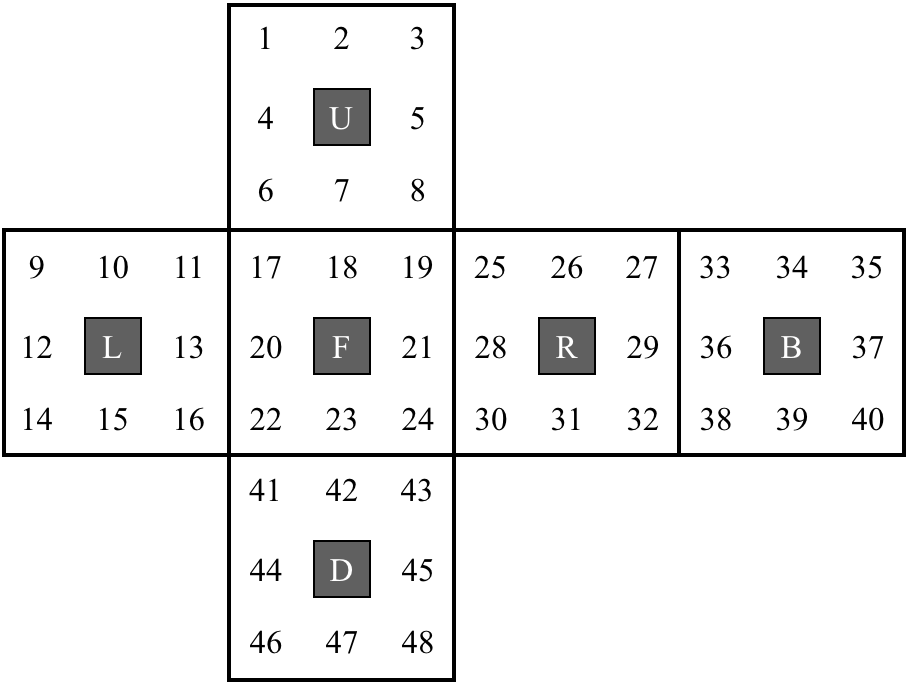
\includegraphics[scale=.24]{numbercube.png}
\caption{The 1 to 48 labelling of the Rubik's cube}
\label{fig:labelled}
\end{figure}

An equivalent labelling which will also be referenced is the cubicle notation from Singmasters \cite{Magic}. This just involves using either two or three letter strings for each cubie, for example with the front face looking at the user, 17 in the diagram would correspond to ulf (upper left face). Similarly 24 is drf (down right face), and 18 the top edge cubie is uf (upper face).
These moves are all of 90 degree, clockwise quarter turns on the cube. Where a solver would be looking at that particular face to make the clockwise move. Throughout the project a move M, would be denoted $M^{-1}$ for an inverse anti-clockwise turn and $M^{2}$ for any half turn move, 180 clockwise turn for $M \in \{L,R,U,D,F,B\}$.

\newpage
\section{Alternating and Symmetric Groups}
Let $X$ be a set and let $S(X)$ be the symmetric group on $X$, the elements of $S(X)$ are the permutations of $X$ (i.e. bijections $X\rightarrow X$) and the group operation is
composition of maps.
In contrast an Alternating group $A(X)$ only contains the permutations to which are just even cycles, as opposed to the symmetric group above containing even and odd cycles. For notation purposes these two groups will be defined as $A_{n}$ and $S_{n}$. \newline A useful map to consider is the group homomorphism operation. This homomorphism will prove to be very useful in later conjectures, and has the following properties:
%Trivially the alternating group $A_{n}$ is contained in the kernel of the map , as it's the even cycles to which are the elements all are mapped to 0. (The kernel just gives the elements mapped to zero by the function).

\begin{align*}
\phi : G\rightarrow H\ \ a&\ \text{group homomorphism where}\\
&\imF(\phi) = \{\phi(a) | a \in G\}\\
&\kerF(\phi)= \{a\in G |\phi(a) = e'\}
\end{align*}
This is where $\kerF(\phi)$ is the kernel of the map and $\imF(\phi)$ is the image of the map. The kernel of a map defines all the elements mapped to the identity, whereas the image is a subset of the range (all the elements mapped to), the output of the function.
In the case for the cube one can define a function below which will map the elements of $S_{n}$ to either 1 or -1 in the cases outlined in the definition below.
\begin{equation}
\phi : S_{n} \rightarrow \{-1,1\} \qquad
  \phi(x)=\begin{cases}
    1, & \text{if x is an even number of transpositions}.\\
    -1, & \text{if x is an odd number of transpositions}.
  \end{cases}
\end{equation}
When x $\in \phi(x)$ equals 1, it means it can be expressed as an even number of transpositions, where transpositions are defined as the 2-cycle permutations. To show the well-defined property of this map, one needs to first show all permutations in $S_{n}$ can be written as a product of transpositions.%INSERTPROOF%% 
This can be shown by the following inductive argument. The base case for $S_{2}$ is trivial. Suppose any permutation of n takes less than n transpositions. Consider a permutation w of length n+1 (transpositions). Using the base case we can perform one transposition to swap the $n+1^{st}$ element in the correct place. Thus by the inductive hypothesis we have less than n transpositions for the remaining n elements, making the total less than n+1 transpositions. 
Now this is known the map can be shown to be a homomorphism by the following.

\begin{prf}{prf:homomproof}

The map can easily be verified to satisfy the conditions above. It is well defined, it can be expressed as some product of transpositions by the proof above.\newline Take two elements $\sigma , \tau \in S_{n}$. The goal is to show $S_{\tau\sigma} = S_{\tau}\cdot S{\sigma}$\newline Either of these can be written like so $\sigma = \alpha_{1} ... \alpha_{a}$ ,$\tau = \beta_{1} ... \beta_{b}$, with some integers a and b factorisations of $\alpha$ and $\beta$ as a product of transpositions.\newline $\sigma\tau = \alpha_{1} ... \alpha_{a}\beta_{1} ... \beta_{b}$ now expresses $\sigma\tau$ as a product of a+b transpositions.\newline $\phi(\sigma\tau)\ =\ (-1)^{a+b}\ =\ (-1)^{a}(-1)^{b}\ =\ \phi(\sigma)\phi(\tau)$
,thus the conditions of a homomorphism is satisfied.
\end{prf}
As the map is known to be a homomorphism, the kernel $\kerF(\phi)$ of the map is of the form $\{a \in g|\phi(a) =e'\}$ where e' is the identity element of the set $\{-1,1\}$. For this case  the identity of the set cannot be 0, as a norm for other groups such as $(\mathbb{Z},+)$,$(\mathbb{N},+)$ as the 0 element does not exist. So the identity shall be defined as the elements of even cycles (odd transpositions), which map to -1. So trivially $A_{n}\subset \kerF(\phi)$, but also it's true that it's the entire kernel, so $A_{n} = \kerF(\phi)$, if it wasn't then for some $S_{n} \notin A_{n} \in \kerF(\phi)$. However this cannot be the case as only even cycles are mapped to -1, and any even cycles in $S_{n}$ are in $A_{n}$ by definition.
Next consider the Group Homomorphism Theorem, or alternatively the First Isomorphism Theorem. 
	

\begin{theo}[Group Homomorphism Theorem]{thm:GHT}
if $\phi: G \rightarrow H$ is a surjective group homomorphism then $G/ker(\phi)\ \cong\ im(\phi)$
\end{theo}


This shows that the group G quotioned out (/) by the kernel is isomorphic to the image of the group. This theorem can be applied to the map $\phi: S_{n} \rightarrow \{-1,1\}$, where it will be shown later that this map is indeed surjective. Substituting the values above defined for the kernel and the image of the group concludes the following: 
\begin{equation}\label{GHT}
S_{n}/A_{n} \cong \mathbb{Z}_{2}
\end{equation}
The cyclic group $\mathbb{Z}_{2}$ is placed at the end as it is equivalent to the set of $\{1,-1\}$ with just two elements, x and the identity (as x is the 1 and the identity has already been defined to be -1).
\paragraph{}From the Group Homomorphism Theorem there is now a new collection called a quotient group, but to understand what a quotient group is to groups one must first consider the left and right cosets formed by each corresponding group.	
With G a group and H a subgroup of G the left and right cosets are as follows:
\begin{itemize}
\item gH = $\{gh\ |\ h \in H\}$ is the left coset 
\item Hg = $\{hg\ |\ h \in H\}$ is the right coset 
\end{itemize}
The subgroup H is just the smallest group contained in G which generates all the elements of H. Taking H = $\{R\}$ (the right turn) as an example, H is now the subgroup of $\mathcal{G}_{RC}$ (the Rubik's cube group), generated by all right turns as shown. 

\begin{figure}[hbt]
\centering%
  \RubikCubeSolved%
  \ShowCube{2cm}{0.5}{\DrawRubikCubeRU}
    \hspace{.4cm}
    \quad\Rubik{R}%
    \hspace{.4cm}
    \RubikRotation{R}
  \ShowCube{2cm}{0.5}{\DrawRubikCubeRU}
  	\hspace{.4cm}
    \quad\Rubik{R}%
    \hspace{.4cm}
   \RubikRotation{R}
   \ShowCube{2cm}{0.5}{\DrawRubikCubeRU}
   	\hspace{.4cm}
    \quad\Rubik{R}%
    \hspace{.4cm}
   \RubikRotation{R}
   \ShowCube{2cm}{0.5}{\DrawRubikCubeRU}
\end{figure}
This is one instance of a right coset purely by definition on the original group $\mathcal{G}_{RC}$. It is such that whatever the size of the subgroup H, it is identical to size of the coset. This is by construction as there is one element in the coset for each element in the subgroup.
It can also be said that any two cosets in a subgroup H constructed from the group G, must be either distinct or the same. So any subgroup must have disjoint cosets, making them unique in definition. This can be shown by a simple proof by contradiction.
\begin{prf}{prf:cosetproof}
\item Suppose there were two right cosets Hx and Hy which share elements.
\item $h_{1}x$ = $h_{2}y$ for some $h_{1},h_{2} \in H$
\item ,taking inverses x = $h_{1}^{-1}h_{2}y$, $h_{3} = h_{1}^{-1}h_{2}$
\item ,giving x = $h_{3}y$ and hx = $hh_{3}y$.
\item So every element of Hx can be written as one of Hy,
\item and so every element of Hx is in Hy, thus Hx= Hy
\end{prf} These such right cosets will partition the Rubik's cube group into equal sized disjoint sets. As the kernel of $\mathcal{G}_{RC}$ is a group itself, the number of distinct cosets is the size of the quotient $|G|/|ker(\phi)$. This is by Lagrange's Theorem.
\begin{theo}[Lagrange's Theorem]{thm:Lagrange}
For H a subgroup of a group G , the size of H must be a divisor of the size of G.
So $x|H| = |G|$ for some $x\geq1$
\end{theo}
So now there is the quotient group $S_{n}/A_{n}$ which is isomorphic to $\mathbb{Z}_{2}$ and of order dividing the Rubik's cube group $\mathcal{G}_{RC}$ by Lagrange. Now whats left is to show is that the map $\phi : S_{n}/A_{n} \rightarrow \{1,-1\}$ preserves a homomorphism as above. As the alternating group has been defined as the kernel above, the group operation (multiplication) will hold in a similar way to the $\phi : S_{n} \rightarrow \{1,-1\}$ map. There are 4 possible occurrences of multiplication in this map defined below.
\begin{align*}
\text{$x$ is even, $y$ is even} \qquad	&\phi(xy) = \phi(x)\phi(y) = 1\cdot1 = 1\\
\text{$x$ is even, $y$ is odd} \qquad	&\phi(xy) = \phi(x)\phi(y)= 1\cdot(-1) = -1\\
\text{$x$ is odd, $y$ is even} \qquad	&\phi(xy) = \phi(x)\phi(y)= (-1)\cdot1 = -1\\
\text{$x$ is odd, $y$ is odd} \qquad	&\phi(xy) = \phi(x)\phi(y) = (-1)\cdot(-1) = 1
\end{align*}
Note by x is even, y is odd, means for x to be defined as an even number of transpositions and y to be odd number of transpositions respectively. So the homomorphic property of multiplication holds, thus the map must be homomorphic.\newline While presently this may not seem that important this conclusion will be paramount in defining the analysis of the cube. This will be referenced later on in the project after valid configurations have been defined.


%group $S_{n}/A_{n}$ is isomorphic to the set containing 0 and 1. As a further argument this set containing 0 and 1 is identical to saying the cyclic group $Z_{2}$, which contains either 0 (the identity), or 1.Group operation is defined similarly , and $({0,1}, +(mod2)) = Z_{2}$ , as two evens cycles still give an even \textcolor{red}{PROP A3 LATEST LINK PROVE}(e.g. 2=0mod2, 2+2=0mod2 ..) as well as any two odd cycles (1+1=2=0mod2) , which mean by group definition both will result to 0 in  the map defined, and 0 (identity) using modulus in $Z_{2}$.Note: this still complies with the definition that the kernel is just the alternating groups as any one even cycle can be written as the product of transpositions of two odd cycles.
\newpage
\subsection{Orienting Precisely}

Now this theory can be related to the example of the 3 by 3 cube. Consider the move $DR^{-1}$ on the start configuration of the cube.


\begin{figure}[hbt]
\centering%
  \RubikCubeSolved%
  \ShowCube{2cm}{0.5}{\DrawRubikCubeRU}
    \hspace{.4cm}
    \quad\Rubik{D}%
    \hspace{.4cm}
  \RubikRotation{D}
  \ShowCube{2cm}{0.5}{\DrawRubikCubeRU}
  	\hspace{.4cm}
    \quad\Rubik{R}%
    \hspace{.4cm}
   \RubikRotation{R}
   \ShowCube{2cm}{0.5}{\DrawRubikCubeRU}
\end{figure}
Only considering the corner cubies for now, labeling them appropriately will allow for the moves to be expressed as a combination of disjoint cycles. For this example just consider the corner cubies numbered 1 to 8. The group considered when making these permutations is the group of all corner cubies $\mathbb{Z}_{3}^{8}$. This is equivalent to the labelling in figure \ref{fig:labelled} where $x_1$ encapsulates the 19,25,8 faces, $x_2$ the 17,11,6 faces and so on in a clockwise fashion.

\begin{equation}
D(\theta)= (1)(2)(3)(4)(5\ 6\ 7\ 8) \ \ \ \ \ \ \ R^{-1}(\theta)= (1\ 7\ 8\ 4)(2)(3)(5)(6)
\end{equation}

The above are the cycles of the Down and Right inverse moves which can be combined to obtain the new move. 
\begin{equation}
DR^{-1}(\theta) = (1\ 8\ 4)(5\ 6\ 7)
\end{equation}

Now the result of this combination is a cycle which alternates the position of the 6 cubies listed above. However this doesn't really achieve anything when looking to solve the cube, as far as the user is concerned this is just any random move $M \in G$. Aiming for a set of moves which oriented 2 cubies for instance would be far more useful in proving properties of the corner cubies and it's corresponding group $\mathbb{Z}_{3}^{8}$. Taking the inverse of the move above, $D^{-1}R$, one obtains a similar disjoint cycle set of, 
\begin{equation}
D^{-1}R(\theta) = (1\ 7)(5\ 8)
\end{equation}

These cycles are in fact isomorphic, which there is a combination that actually achieves the aim. Through inspection applying the moves together the combination is as follows:

\begin{equation}\label{orientcorner}
(DR^{-1}D^{-1}R)^{2}  U^{-1}  (DR^{-1}D^{-1}R)^{4} U 
\end{equation}

\newcommand{\OrientingCorner}{[Orienting Corners],D,Rp,Dp,R,D,Rp,Dp,R,Up,D,Rp,Dp,R,D,Rp,Dp,R,D,Rp,Dp,R,D,Rp,Dp,R,U}%
\newcommand{\OrientingCornerArrow}{$\quad\overrightarrow{\strut\textsc{Orienting the corners}}\quad$}

\begin{figure}[h]
\centering
  \RubikCubeSolved%
  \ShowCube{2cm}{0.5}{\DrawRubikCubeRU}
  \RubikRotation{\OrientingCorner}
  \quad\SequenceBraceA{\SequenceName}{\ShowSequence{}{\Rubik}{\SequenceLong}}
  \ShowCube{2cm}{0.5}{\DrawRubikCubeRU}
\end{figure}

But this inspection doesn't seem very trivial and leaves the question where is the intuition and maths behind such a move. For this explanation it's useful to turn to commutators from Group Theory. 
\begin{equation}
\text{The commutator of two elements, } g \text{ and } h, \text{of a group } G\text{, is the  element} :\ ghg^{-1}h^{-1}
\end{equation}

For the cube this can be translated by setting g,h to be a specific set of moves. So really what's done above is to find the commutator which orients the two corner cubies by using the definition of a commutator. Where instead of considering disjoint cycles, defining g and h like so,

\begin{equation}\label{orient}
	g = R^{-1}DRD^{-1}R^{-1}DR\ \ \ \ \ \ 
    h = U^{-1}
\end{equation}
and applying the commutator algorithm $(ghg^{-1}h^{-1})$ gives the set of moves to orient two corner cubies again. The importance of these commutators is high as it allows the user to gain intuition into actually solving the cube rather than just following a set algorithm. This also becomes particularly useful when the cube is a few moves off the start configuration and say the user needs to permute two corner cubies, now with the knowledge of the correct group commutator this can be achieved. Along with orienting the corners implementing these commutators give a lot of useful moves, such as swapping edge pieces, corner 3-cycles and so on. These such moves will be discussed later in generating the cube.

\section{Generating the Cube}
\subsection{Generators and Orbits}
Let G be a group, a subset $S\subseteq G$ is a generating set of G if $G =\langle S\rangle $. In other words every element of G can be written as a finite product (under group operation) of elements of S. These elements are called generators of G. Taking the group G to be composed of the 6 basic moves  $G= \{{F,L,R,U,D,B}\}$, such that  any cube permutation can be made, allows a comparison to be made of what a generator means to this specific example. For example taking $S=\{R\}$ gives the subgroup which obtains all possible cube permutations obtained by rotating the right face $\{R,R^2,R^3,R^4\}$. As the order of a group is defined as either the least $n \in \mathbb{N}$ such that $g^n = \epsilon$ (where g is a member of the group),  or alternatively the size of the subgroup it generates, the order for S will be 4. Note it stops at $R^4$ as the group is cyclic*, so $R^5= R$.*by cyclic it just means to say that there exists an element which creates a generating set.\newline In group theory many groups share the property of being Abelian, which means for a group (G,*) if $\forall x,y \in G,\ x*y=y*x$. One example could be $(\mathbb{Z},+)$ the group of the integers on addition, for any integer $x,y$ this will hold (3+4 = 4+3) as the integers are commutative and associative in definition.
However applying this to the Rubik's cube group this will not hold, showing us the order in which the moves are applied does in fact matter. This is shown by a simple case of the move M = $\{L,R2,D\}$ below.

\begin{figure}[h]
\centering
  \RubikCubeSolved%
  \RubikRotation{L}\RubikRotation{R2}\RubikRotation{D}
  \ShowCube{2cm}{0.5}{\DrawRubikCubeRU}
  \RubikCubeSolved%
  \RubikRotation{R2}\RubikRotation{D}\RubikRotation{L}
  \hspace{.4cm}
  \ShowCube{2cm}{0.5}{\DrawRubikCubeRU}
\end{figure}
Where, from the starting configuration, the left hand cube has been applied the sequence ${L,R2,D}$ and the right hand cube ${R2,D,L}$. Visually one can see the are obviously not equal, thus breaking the condition of what it means to be abelian. This is because these moves share common cubies, a move consisting of opposite faces alone such as R,L would hold commutativity (RL=LR) however for the whole cube this can't be said. So clearly some elements of the group commute while others do not.\newline The set of elements to which the generators are made from is defined as the generating set. These generators are a useful way for defining groups, however for large groups such as the Rubik's cube it can become difficult to gain information due to the sheer enormity of possible generators. When talking about these commuting elements it's often useful to mention orbits and their stabilisers. 

Consider the definition of an orbit from Group Theory.
\begin{defn}[Orbit]{defn:orb}
if G acts on a set A, then the orbit of a $\in$ A (under this action) is the set $\{a*g:g \in G\}$ 
The stabiliser of an orbit is $\{g\in G | g*x = x\}$ the set of all elements that fix x
\end{defn}

The orbit is just the subset of A which can be moved by any move on G, with A being the total number of configurations of the cube. As said above the center cubies always stay in the 6 center positions hence will always be in the same orbit. This applies to the corner and edge cubies as well (relative to corner and edge positions). 
From properties of an orbit, it must be either disjoint or the same (this can be shown from a single contrapositive argument). So one could consider 3 separate orbits within the Cube where,

\begin{equation}
A = A_{x}\cup A_{e}\cup A_{c}\cup A_{e}
\end{equation} 
$A_{x}$ are the center pieces, $A_{e}$ edge pieces and $A_{c}$ the corner pieces. We know any of these cubies will stay in their respective positions from a move G, but what isn't so is trivial is when one considers the whole set of the cubies. Moreover prove how any group action from the Rubik's Group $\mathcal{G}_{RC}$ preserves that any resulting configuration will be in the same orbit. 
An example of when the wouldn't apply is any illegal configuration of the cube (e.g. from pulling pieces out, switching stickers etc.), defining the difference into what is and isn't a valid configuration is key in proving the statement about orbits above. This will be referenced later in the paper.
Orbits aswell as describing how points, or in the case described, cubies move can also be used to compute stabilisers. These can be the subgroups of elements which fix one or more points, which can be very useful in solving the cube in a step by step solution\cite{PermGroups}.\newline Suppose there was an algorithm which took a given scrambled state to the starting configuration. Where in this algorithm one piece has been permuted correctly, call it $G_{1}$, where the rest of the cube remains to be solved. These subsequent permutations will aim to put their respective pieces in the correct place (and orientation) without disturbing the previous permutation.   

This algorithm is called a stabiliser chain where the first permutation fixing the first piece of the cube, $G_{1}$ shall be defined as the stabiliser of the chain. $G > G1 > G2 > .... > Gn = I$, where I is the identity (starting configuration).Each of these $G_{i}'s$ should contain a set of moves which solves the i'th piece, therefore one of the move sequences for that $G_{i}$ will be in $G_{i+1}$, a permuation in $G_{i}$ will always lie in $G_{i+1}$. In other terms with a list  of a move $a_{i1},a_{i2},a_{i3}, ...$ every $b \in G_{i} \in a_{ik}G_{i+1}$ for some k. So $G_{i}$ is made up entirely of the set of all cosets $a_{i1}G_{i+1}, a_{i2}G_{i+1}, a_{i3}G_{i+1}, ... $ for every k. There now exists a way to find the generators for $G_{i+1}$ a specific sequence solving the ${i+1}^{th}$ piece, that given the generators of $G_{i}$ and the list of move sequences $a_{ik}$ (or coset representatives), the new stabiliser chain can be built\cite{Schreier}.

The Rubik's cube group $\mathcal{G}_{RC}$ if to be implemented by a computer using each individual configuration, which is $(8!\cdot 3^8\cdot 12!\cdot 2^12/3\cdot 2\cdot 2) \approx 4.3\cdot 10^{19}$, becomes computationally inefficient to try and store each solving sequence for each configuration. The aim of implementing the following algorithm however is to identify the groups composition structure by using subgroups to factorise the problem down, to solve the cube from a given state. The algorithm in question the Schreier Sims Algorithm, is given motivation from the Schreier Lemma on subgroups.

\begin{lem}[Schreier Lemma on Subgroups]{lem:Schreoer}
Let G be a group with a set of generators S. Let H be a subgroup of G, and let A be the set of coset representatives of H $\in$ G. For any g $\in$ G, let g denote the element of A that represents the coset gH.\newline Then H is generated from the set $\{(sa)^{-1} (sa) | a \in R, s \in S \}$. 
\end{lem}

\begin{prf}{prf:schreier}
Take any $h\in H (\in G)$ , $h = s_{1}s_{2}...s_{k}$ for some sequence of generators $s_{i} \in S$.
\[Let\ \ \ t_{i} = s_{i+1}...s_{k}\ \ \ be\ the\ coset\ representative\ for\ the\ s\ sequence\] This is such that $t_{0}$ = $s_{1}...s_{k}$ = $h$ and $t_{k}$ defines the identity $t_{k} = e$.
Rewriting $h$ with new set of coset representatives $t$ gives $h$ = $(t_{0}^{-1} s_{1} t_{1}) ...(t_{k-1}^{-1} s_{k} t_{k})$.
One also finds that $(s_{i} t_{i})H = s_{i}(t_{i} H) = s_{i} ( s_{i+1}..s_{k} H) = (s_{i}s_{i+1}..s_{k})H = t_{i-1} H so s_{i} t_{i} = t_{i-1}.$
Rewriting $h$ with this new condition gives $h = ((s_{1} t_{1})^{-1} s_{1} t_{1})((s_{2} t_{2})^{-1} s_{2} t_{2}) ...((s_{k} t_{k})^{-1} s_{k} t_{k})$.
By definition $t$ is the set of coset representatives, giving each $i$ interval a factor of $s_{i}^{-1}s_{i}$. Any element $h \in H$ is a product of these factors, thus the set $\{(sa)^{-1} (sa) | a \in R, s \in S \}$ will generate H.\\
\end{prf}
The method to factorise into smaller subgroups uses a combination of Lagranges Theorem with the Orbit Stabiliser Theorem. 
\begin{theo}[Orbit Stabiliser Theorem]{thm:Orbit}
Let G be a group which acts on a finite set X. For each $x \in X$, with $Gx$ the orbit, $G_x$ the stabiliser of $x \in G$, then $|G|= |Gx|*|G_{x}|$\ and applying Lagrange gives \\ $|Gx|=|G/G_{x}|=|G:G_{x}|$
\end{theo}

This simply states the size of the orbit of the group can be retrieved from the size of the group partitioned by its stabilisers. Any subgroup chain can also be completed in $log_{2}|G|$ as the stabiliser is a subgroup for the rubiks cube group ($G>G_{x})$ meaning $[G:G_{x}]\geq 2$, so $|G|\geq2|V|$ and $|G|\geq 2^{k}.$\cite{OrbStab}. So reducing the problem logarithmically can cause a major difference to understanding an algorithm to solve the cube in a certain state in the orbit, however the reduction is not that significant as $[G:G_{x}]$ still remains very large. In fact for each predecessing $G_{i}$ the number of generators grows exponentially, $G_{1}$ = 6*24, $G_{2}$=6*24*22 . . . For an efficient solver one would need to extract which of these generators are useful to the solving problem as a large number of these are not. The algorithm has been adapted to improve on these flaws, which along with other solvers shall be mentioned later.
%Incremental Schreier-Sims algorithm.

\subsection{Various Moves and Orders}

Each individual basic move of the rubik cube has generator 4 which can be seen easily by rotating the cube. Below is a list of some other group generators with their factors, where the figure in size shows number of moves to cycle back to the starting configuration \cite{gentable}.

\begin{figure}[h]
\begin{center}
    \begin{tabular}{ | p{7cm} | p{2cm} | p{3cm}|}
    \hline
    Generators & Size & Factor \\ \hline
    U & 4 & $2^2$\\ \hline
    U, RR & 14,400 & $2^6 \cdot 3^2 \cdot 5^2$ \\ \hline
    U, R  & 73,483,200 &$2^6 \cdot 3^2 \cdot 5^2$\\ \hline
    RRLL, UUDD, FFBB & 8 & $2^3$ \\ \hline
    RL, UD, FB & 6,144 & $2^11 \cdot 3$\\ \hline
    FF, RR & 12 &$ 2 \cdot 3^2$\\ \hline
    FF, RR, LL & 96 &$ 2^8 \cdot 3$\\ \hline
	FF, BB, RR, LL, UU & 663,552 &$ 2^13 \cdot 3^4$\\ \hline
    LLUU & 6 & $2 \cdot 3$\\ \hline
    LLUU, RRUU & 48 &$ 2^4 \cdot 3 $\\ \hline
    LLUU, FFUU, RRUU & 82,944 &$ 2^{10} \cdot 3^4$\\ \hline
    LLUU, FFUU, RRUU, BBUU & 331,776 &$ 2^{12} \cdot 3^4 $\\ \hline

    \end{tabular}
\end{center}
    \caption{Size of various subgroups of the Rubik's cube group}
    \label{fig:movestable}
\end{figure}
From the table there is no real apparent direct correlation between the length of the move sequence and the (size) distance from the cube. This can be seen especially when considering the two generating set $\langle U,R\rangle$. This is an important generator for the group while most other generators will only produce smaller size subgroup, $\langle U,R\rangle$ can be seen to generate the entire Rubik's cube group.

\subsection{Minimally Generating Set}

The Rubiks cube is generated by the set of basic moves M = $\{L,R,U,D,F,B\}$ where one can reach each configuration from a combination of these. However it actually stands that this set of moves M is not minimal and in fact the rubiks group can be generated by just 5 of these moves, $M^{'} = R,L,F,B,U$ \cite{bandelow2012inside}. With this set the move D and $D^{'}$ can be simulated using $M^{'}$ by doing the following two moves found by Roger Penrose:
\begin{align*}
D &= R^{2}L^{2}U^{-1}B^{2}F^{2}U^{-1}B^{2}R^{2}B^{2}F^{2}L^{2}F^{2}U^{-1} \\
D^{-1} &= R^{2}L^{2}UF^{2}B^{2}UF^{2}R^{2}F^{2}B^{2}U^{2}L^{2}U^{2}L^{2}R^{2}U^{2}R^{2}U^{2}R^{2}F^{2}U^{-1}R^{2}B^{2}R^{2}L^{2}F^{2}L^{2}UB^{2}F^{2}U
\end{align*}

The downside to using this set is the efficiency when implementing the down moves using these replacements. However one cannot dispense another standard generator, 5 of the basic moves are needed.

\subsection{2-Generated Group}

The Rubiks Cube group is a 2-generator group meaning that choosing any two elements of the cube will give a high chance of generating the whole group (p32) \cite{Magic}. Frank Barnes observed this using the two moves below.
\begin{align*}
\alpha &= L^{2}BRD^{-1}L^{-1} &= (RF,RU,RB,UB,LD,LB,LU,BD,DF,FL,RD)\\& &(FUR,UBR,LDB,LBU,DLF,BDR,DFR) \\
\beta &= UFUR^{-1}U^{-1}F^{-1} &= (UF,UL)_{+}(UR)_{+}(UBR,UFL)_{-}(URF)_{+} 
\end{align*}
Here the notation slightly differs from the usual disjoint-cycle so shallbe explained here. A move with the two character (LU,BD) is an edge cycle. This will move the LU edge piece to the BD edge cubie such that position of L will move to half end up in the B face, and U doing a similar action with D. Notation for a corner is similar with the corresponding 3 character cycles e.g. (URF URB). Finally $(UF,UL)_{+}$ is called a twisted cycle, taking the UF cubie to the UL position however the final edge cubie orientation flips when cycling back. Again for a corner this is similar where the cubie is rotated to the next face when cycling back.\newline The element $\alpha^{7}$ is an 11-cycle of edges and $\alpha^{11}$ is an 11-cycle of corners, generating the orientation subgroups which wil be mentioned in the next section. $\beta$ will act on the edges and corner cubies that $\alpha$ fixes. The fact that these 2 elements genrate the whole group can now be verified much easier with the implementation of cube related languages like GAP \cite{GAP}.


%INSERT SOMETHING MAYBE ABOUT 2X2 CUBES ON THE REFERENCE


\pagebreak
\section{Possible and Non Possible Configurations}


We have the orientations of a corner cubie defined as $\mathbb{Z}_3$.
This is because each of corner cubie has 3 coloured faces which can be oriented differently. 
This makes the set of 8 corner cubies the product of all these different permutations.\[\mathbb{Z}_{3}^8 = \prod_{i=1}^{8}\mathbb{Z}_{3}\]
To think about the different orientations of a cubie the idea is to fix a 'starting orientation' .We know there must exist a homomorphism which takes the cubies to the correct orientation , as there exists a set of moves leading any valid configuration to the start configuration (solved). Thus using the group $\mathbb{Z}_{3}^{8}$ , generators of such group would be basis elements,  so fixing 7 cubies gives the homomorphism below: 

\begin{align}
	\delta : G \Rightarrow G && \delta(\mathbb{Z}_{3}^{7}) = \epsilon
\end{align}

Also when considering the subgroups of $\mathcal{G}_{RC}$, it's necessary to define another subgroup along with the orientations of the cubies, this being $S_{8}$ the permutation group of 8 elements (the 8 corner cubies). This can be defined like such, as taking any corner cubie on the cube it has 3 faces as described above which can all be alternated between each other. This being equivalent to a 3-cyclic group, denoted $C_{3}$. Which leads again to a product of 8 groups \[\mathcal{C}_{3}^8 = \prod_{i=1}^{8}\mathcal{C}_{3}\], where $C_{3}^{8}$ can be found to make up $S_{8}$. These 2 definitions above analogously follow a similar argument when considering the 12 edge cubies along the cube $\mathbb{Z}^{12}_{2}$.
\paragraph*{}
Going back to orbits and considering the difference between correct configurations, notation on what defines a valid configuration is necessary. At any configuration all corner cubies, as well as edge cubies, should be on orientation number corresponding to that of their group. That is,
\begin{align*}
e.g.\ \ x_1&=0,\ x_2=2\ ...,\ x_8=1\\
y_1&=1,\ y_2=1\ ... ,\ y_{12}=0
\end{align*}
One must also define a sign variable which states what the move has done to change the orientation of the corner cubies, or that of the edge cubies. 
Define $\tau (\in S_{8})$ as the sign of the corner cubies and $\delta (\in  S_{12})$ as the sign of the edge cubies. This sign is 1 if there is an even number of transpositions, which are 2-cycle permutations, and -1 if there is an odd number. 
\begin{equation}
  \tau(x)=\begin{cases}
    1, & \text{if x contains an even number of transpositions}.\\
    -1, & \text{if x contains an odd number of transpositions}.
  \end{cases}
\end{equation}

Note a k-cycle or k-cycle permutations are just cycles which have k length (k elements).\newline Ignoring the center cubies as they always stay in the same position relative to the cube, a configuration is defined as \textbf{$(\tau,\delta, x, y)$ }.
For example an invalid configuration would be that in figure \ref{fig:invalid}.

\newcommand{\invalidseq}{[invalidseq],F2,F2}%
\newcommand{\invalidseqarrow}{$\quad\overrightarrow{\strut\textsc{invalidseq}}\quad$}

\begin{figure}
\centering
  \RubikCubeSolved%
  \ShowCube{2cm}{0.5}{\DrawRubikCubeRU}\invalidseqarrow
  \RubikRotation{\invalidseq}
  \RubikFaceUp   {W}{W}{W} {W}{W}{W} {W}{W}{G}%
  \RubikFaceFront{O}{O}{W} {O}{O}{O} {O}{O}{O}%
  \RubikFaceRight{O}{G}{G} {G}{G}{G} {G}{G}{G}%
  \ShowCube{2cm}{0.5}{\DrawRubikCubeRU}
\caption{Impossible move sequence taking the cube to invalid configuration}
\label{fig:invalid}
\end{figure}
\vspace{20pt}
This is because there exists no set of moves to obtain the configuration shown on the right. The change of orientation of one singular cubie (from the start configuration) can only be achieved by breaking the cube, so is invalid. Given the definitions of a configuration and the labelling previous in figure \ref{fig:labelled}, this can be shown mathematically. 

%To show this apply the following:

To see if one configuration can be found from another is identical to saying $(\tau^{'} ,\delta^{'} , x^{'} , y^{'} )$ = $(\tau,\delta, x, y) \cdot$ M e.g. applying a move M gives the different configuration. Using knowledge of orbits, define it to be the set of all possible configurations from the Rubik's Cube group $\mathcal{G}_{RC}$. It's known whenever a move M applied to a possible configuration is also valid then one can conclude any other valid configuration can be found from a move M. As this trivially holds for any one of the basic moves $M= \{{F,L,R,U,D,B}\}$, one can conclude using inductive principles, that for any intermediate set of moves this will still hold, as the new configuration will still be in the orbit. Giving reason to saying any valid configuration of the cube can be solved with a specific set of moves. However to prove one of the fundamental theorems on the cube, the corresponding signs of two correct configurations must be evaluated, hence we define the two following maps.


\begin{equation}\label{onto}
\phi_{corner}: G \rightarrow S_{8}\quad \quad 
\delta_{edge}: G \rightarrow S_{12}
\end{equation}
This maps all elements of the group to the subgroup $S_{8}$ (Symmetric group of the corner cubies). This map is a homomorphism as it is trivially well defined, and preserves the group operation of a move e.g. $\phi (L \cdot L) = \phi (L) \cdot \phi(L)$. With this homomorphism the above objective, $(\tau,\delta, x, y) \longrightarrow (\tau^{'},\delta^{'}, x^{'}, y^{'})$ from $\tau^{'} = \tau\phi_{corner}(M) $, and similarly with edge pieces $\delta^{'} = \delta\phi_{edge}(M) $ works as from the following proof:

It's known that the homomorphism is surjective, otherwise there would exist possible moves in $M= \{{F,L,R,U,D,B}\}$ taking corner cubies out of the subset of corner cubie positions (contradicting our definition of the orbit of the cube group). This trivially cannot happen, a cubie with 3 faces cannot live in an edge cubie consisting of 2 faces, meaning any application of $\phi_{corner}: G \rightarrow S_{8}$ will result in one of the 8 corner cubies. Below will formally show that this is in fact a surjective homomorphism: 
\begin{lem}[Surjectiveness]{lem:surject}
The homomorphism $\phi_{corner}: G \rightarrow S_{8}$ between the rubiks cube group G and the symmetric group $S_8$ is surjective
\end{lem}
\newpage
\begin{prf}{prf:surjective}
It's known the symmetric group $S_8$ is generated by the set of 2-cycles in $S_8$ as well as that for any $n$ (in $S_n$). So to show surjectivity it's equivalent to show every 2-cycle (in $S_8$) is in the image subgroup $\imFD_{\phi_{corner}}$. This just means the image is entirely those 2-cycles which make up the corner cubies, and hence would mean $\sgnF(\tau) = 1$.
By taking any such commutator of the cube, and using trial and inspection on a said amount of cycles, a move switching position of two corner cubies (while leaving the other corners fixed) can be found. One such move is M = $([D,R]F)^{3}$ with the commutator [D,R]. This takes $x_3$ to $x_8$ making the cycle $(x_3\ x_8)$ while also switching edge cubies as there exists no move solely switching two corner cubies without affecting any of the other cubies. With this move applied to the map it gives $\phi_{corner}(M) = (x_3\ x_8)$ thus $(x_3\ x_8)$ must lie in the image of $\phi_{corner}$, it just remains to show the others do as well.\newline Take $x_i$, $x_j$ as any two corner cubies, any corner cubie can be placed in the position of another so there must exist a move p sending $x_3$ to $x_i$ and $x_j$ to $x_8$.Let $\sigma =\phi_{corner}$ and as $\phi_{corner}$ is a homomorphism the following applies:
\begin{align*}
\phi_{corner}(p^{-1}Mp) &= \phi_{corner}(p)^{-1}\phi_{corner}(M)\phi_{corner}(p)\\
		&= \sigma^{-1}(x_3\ x_8)\sigma			\\
		&= (\sigma(x_3)\ \sigma(x_8)) &&\text{As $\sigma^{-1}(x_i ... x_ k)\sigma = (\sigma(x_i) .. \sigma(x_k))$} \\
&= (x_i\ x_j) &&\qedhere
\end{align*}
So for any $x_i$ and $x_j$ distinct in $\{x_1,...,x_8\}$ $(x_i\ x_j)$ is in the image of the map, moreover $(x_i\ x_j) \in \imFD_{\phi_{corner}}$.
\end{prf}
 In having a surjective homomorphism, the Group Homomorphism Theorem can be applied once again (theorem \ref{thm:GHT}) by inspection the kernel of this group is empty thus the image is equivalently $S_{8}$. Any $\tau$ $\in S_{8}$ of this new image subgroup ($S_8$) can be described as an element which moves the corner cubies from their start positions to the new positions. From the way $\tau$ is defined it shall be either 1 or -1, using the homomorphic properties of $S_{8}$ must contain an inverse element (for every element in the group), meaning applying one of the basic moves M, one can get cubie A to its original position from its new position. One of these basic moves permutes 4 corner cubies, making the permutation a 4-cycle, thus being an even number of transpositions $\tau^{'}$ = 1. Which also means $(\tau^{'} ,\delta^{'} , x^{'} , y^{'} )$ = $(\tau,\delta, x, y) \cdot$ M, hence $\tau^{'} = \tau\phi_{corner}(M)$. So if $\tau^{'} \neq \tau$ e.g. $\tau = -1$ applying M means $\tau$ will now alter from an even to an odd number of transpositions thus $\tau = -1 \cdot -1 = 1$ and $\sgnF(\tau^{'}$) = $\sgnF(\tau$).

\newpage

There is an analogous argument with the edge cubies for $\delta^{'} = \delta\phi_{edge}(M) $. Combining the analogous argument and the fact that any basic move M moves 4 corner and 4 edge cubies the following can be concluded:
\begin{prop}[]{prop:4cycle}
For any basic move $M \in \{L,R,U,D,F,B\}$, which takes a configuration to it's new state $(\tau^{'} ,\delta^{'} , x^{'} , y^{'} )$ = $(\tau,\delta, x, y) \cdot$ M. The product of the signs will remain equal such that $\sgnF(\tau)\sgnF(\delta) = \sgnF(\tau^{'}) \sgnF(\delta^{'})$
\end{prop}
\begin{prf}{prf:4cycle}
\begin{align*}
\sgnF(\tau^{'}) \sgnF(\delta^{'}) &= \sgnF(\tau)\sgnF(\delta) \\ 
		&= \sgnF(\tau)\sgnF(\phi_{corner}(M))\sgnF(\delta)\sgnF(\phi_{edge}(M))&&\text{Using homomorphisms above}  \\
        &= \sgnF(\tau)(-1)\sgnF(\delta)(-1) &&\text{Both 4 cycles}  \\
        &=  \sgnF(\tau)\sgnF(\delta)  &&\qedhere
\end{align*}
\end{prf}
Furthermore as the start configuration is defined as (1,1,0,0) by looking at the definition of the signs, one can say any other valid configuration is also in the start configuration as shown above giving that $\sgnF(\tau) = \sgnF(\delta)$. 
This fact is fundamental in cube theory, but a full definition of what makes a correct configuration is not fully complete. For this conservation of parity between edge and corner cubies must be verified. This touches on the point made earlier in the section discussing that each cubie, edge or corner, must be associated with a number to describe the orientation of the cubie in that specific cubicle. Otherwise mathematically speaking, it cannot be told if the cubes are facing in the right directions. These $x$ and $y$ values must obey the following rules: 

\begin{equation}
\Sigma x_{i} =0mod(3) \qquad \Sigma y_{i} =0mod(2) 
\end{equation}

From the labelling defined previously for $x_{1}$ to $x_{8}$ and $y_{1}$ to $y_{12}$ the basic move M will change these values on one configuration($(\tau^{'} ,\delta^{'} , x^{'} , y^{'} )$ = $(\tau,\delta, x, y)$ * M) in the table below \cite{chengroup}:

\begin{center}
\label{:paritytable}
    \begin{tabular}{ | l | p{12cm} |}
    \hline
    Move & x' and y' value \\ \hline
    D &  $x_1,x_2,x_3,x_4,x_8,x_5,x_6,x_7$ \\
& $y_1,y_2,y_3,y_4,y_5,y_6,y_7,y_8,y_{10},y_{11},y_{12},y_9$\\ \hline
    R &  $x_1,x_7 +1,x_2 +2,x_4,x_5,x_6,x_8 +2,x_3 +1$\\ & $y_1,y_7,y_3,y_4,y_5,y_2,y_{10},y_{8},y_{9},y_{6},y_{11},y_{12}$\\ \hline
    U &  $x_2,x_3,x_4,x_1,x_5,x_6,x_7,x_8$ \\ & $y_4,y_1,y_2,y_3,y_5,y_6,y_{7},y_{8},y_{9},y_{10},y_{11},y_{12}$\\ \hline
    L & $x_4 +2,x_2,x_3,x_5 + 1,x_6 +2,x_1 + 1,x_7,x_8$ \\
& $y_1,y_2,y_3,y_5,y_12,y_6,y_{7},y_{4},y_{9},y_{10},y_{11},y_{8}$\\ \hline
    F &  $x_6 +1,x_1 +2,x_3,x_4,x_5,x_7 +2,x_2 +1,x_8$\\
& $y_1,y_2,y_8 +1,y_4,y_5,y_6,y_{3}+1,y_{11}+1,y_{9},y_{10},y_{7}+1,y_{12}$\\ \hline
    B &  $x_1,x_2,x_8 +1,x_3 + 2,x_4 + 1,x_6,x_7,x_5 +2$ \\
&$y_6 +1,y_2,y_3,y_4,y_1 +1,y_9 +1,y_{7},y_{8},y_{5}+1,y_{10},y_{11},y_{12}$\\ \hline
    \end{tabular}
\end{center}
The method in which the corresponding $x's$ and $y's$ have been added by a number between mod 2 or mod 3 is defined below. Assume the below cube consists of a valid configuration, where there exists a move sequence which rotates the top front face corner cubie in its cubicle only. 

\newcommand{\rotatecorner}{[rotatecorner],F2,F2}%
\newcommand{\rotatecornerarr}{$\quad\overrightarrow{\strut\textsc{rotate corner }}\quad$}
\begin{figure}[hbt]
\centering
  \RubikCubeSolved%
  \RubikFaceUp   {X}{X}{X} {X}{X}{X} {X}{X}{G}%
  \RubikFaceFront{X}{X}{W} {X}{X}{X} {X}{X}{X}%
  \RubikFaceRight{O}{X}{X} {X}{X}{X} {X}{X}{X}%
  \ShowCube{2cm}{0.5}{\DrawRubikCubeRU}\rotatecornerarr
  \RubikRotation{\rotatecorner}
  \RubikFaceUp   {X}{X}{X} {X}{X}{X} {X}{X}{W}%
  \RubikFaceFront{X}{X}{O} {X}{X}{X} {X}{X}{X}%
  \RubikFaceRight{G}{X}{X} {X}{X}{X} {X}{X}{X}%
  \ShowCube{2cm}{0.5}{\DrawRubikCubeRU}\rotatecornerarr
  \RubikFaceUp   {X}{X}{X} {X}{X}{X} {X}{X}{O}%
  \RubikFaceFront{X}{X}{G} {X}{X}{X} {X}{X}{X}%
  \RubikFaceRight{W}{X}{X} {X}{X}{X} {X}{X}{X}%
  \ShowCube{2cm}{0.5}{\DrawRubikCubeRU}
\end{figure}
\vspace{20pt}
Also assume the cubie fits in the cubicle correctly in the first cube, e.g. its in the correct position and orientation currently. Each time a move is applied and the cubie is rotated from it's correct orientation there will be an addition of 1 to preserve notational parity. For example let the cubie = $x_2$, when the rotate corner sequence is applied the orange moves to the white facet clockwise 1 face, so the new $x_2^{'}$ becomes $x_2 + 1$. If the sequence was applied twice to go from the first to the third the new $x_2^{'}$ becomes $x_2 + 2$ as there are 2 clockwise movements. This is also similar for the edge pieces, but for only 2 changing faces there will only ever be a +1 or +0 (cycles back).
As an example the front face turn is shown below.

%INSERT DIAGRAM OF FRONT MOVE

\begin{figure}[hbt]
\centering
\RubikCubeSolvedWY
\ShowCube{5cm}{0.5}{
	\DrawRubikCubeSF
	\node (x1) at (.5, 2.5)
		[black]{\small\textsf{x1}};
	\node (x2) at (2.5, 2.5)
		[black]{\small\textsf{x2}};
	\node (x6) at (.5, .5)
		[black]{\small\textsf{x6}};
	\node (x7) at (2.5, .5)
		[black]{\small\textsf{x7}};
	\node (x3) at (4.5, 3.5)
		[black]{\small\textsf{x3}};
	\node (x4) at (-2.5, 2.5)
		[black]{\small\textsf{x4}};
	\node (x5) at (-2.5, .5)
		[black]{\small\textsf{x5}};
	\node (x8) at (4.5, 1.5)
		[black]{\small\textsf{x8}};
}
\hspace{.5cm}
\Rubik{F}%
\hspace{.5cm}
\ShowCube{5cm}{0.5}{
	\RubikRotation{F}\DrawRubikCubeSF
	\node (x6) at (.5, 2.5)
		[black]{\small\textsf{x6}};
	\node (x1) at (2.5, 2.5)
		[black]{\small\textsf{x1}};
	\node (x7) at (.5, .5)
		[black]{\small\textsf{x7}};
	\node (x2) at (2.5, .5)
		[black]{\small\textsf{x2}};
	\node (x3) at (4.5, 3.5)
		[black]{\small\textsf{x3}};
	\node (x4) at (-2.5, 2.5)
		[black]{\small\textsf{x4}};
	\node (x5) at (-2.5, .5)
		[black]{\small\textsf{x5}};
	\node (x8) at (4.5, 1.5)
		[black]{\small\textsf{x8}};
}
%\caption{F move on solved cube}
\end{figure}
\begin{figure}[hbt]
\centering
\RubikCubeSolvedWY
\Rubik{L}%
\hspace{.5cm}
\ShowCube{5cm}{0.5}{
	\RubikRotation{F}\RubikRotation{L}\DrawRubikCubeSF
	\node (x4) at (.5, 2.5)
		[black]{\small\textsf{x4}};
	\node (x1) at (2.5, 2.5)
		[black]{\small\textsf{x1}};
	\node (x6) at (.5, .5)
		[black]{\small\textsf{x6}};
	\node (x2) at (2.5, .5)
		[black]{\small\textsf{x2}};
	\node (x8) at (4.5, 1.5)
		[black]{\small\textsf{x8}};
	\node (x3) at (4.5, 3.5)
		[black]{\small\textsf{x3}};
	\node (x5) at (-2.5, 2.5)
		[black]{\small\textsf{x5}};
	\node (x7) at (-2.5, .5)
		[black]{\small\textsf{x7}};
}
\end{figure}
Where in the solved position $x_1$ has a white face up, blue face leftwards and orange face frontwards. After the permutation (1,2)(2,7)(7,6),(6,1), it now lives in the $x_2$ cubicle where the blue face is now upwards, the blue face is 2 clockwise positions from initial (white face), thus $x_1$ + 2. The same applies with other cubies affected given after an F move $x_1$ + 2,$x_2$ + 1,$x_6$ + 1,$x_7$ + 2, complying with the table above. Applying an additional L move takes (5,4)(4,6)(6,7),(7,5) to their new positions. Giving $x_4$ + 2,$x_5$ + 1, $x_6$ + 2, $x_7$ +1 and leaving the remaining corner cubies unchanged. Note these x's are taken as permutations from the start configuration not for the previous move.\newline So checking parity of all the corner cubies in this for the new configuration $(\tau^{'},\delta^{'}, x^{'}, y^{'})$ under the move FL:
\begin{equation}
x^{'} = x_1 + 2, x_2 + 1, x_3 + 0, x_4 + 2, x_5 +1, x_6 + 2, x_7 + 1, x_8 + 0
\end{equation}
\begin{equation}\label{sigmasequal}
\Sigma{x_i^{'}} = \Sigma{x_i} + 9  = \Sigma{x_i} (mod 3)
\end{equation}
This will hold for any of the moves as shown in the parity table\ref{:paritytable}, and therefore any subsequent set of moves.
In fact given the above information the conservation for the parity of corner and edge cubies can already be shown.
\begin{theo}[Parity of Edge and Corner Cubies]{parity}
If $(\tau,\delta, x, y)$ is a valid configuration then $\Sigma x_{i} =0mod(3) \qquad \Sigma y_{i} =0mod(2) $
\end{theo}
Because its shown that any permutation of moves leaves the new configuration in the same orbit as the start configuration (1,1,0,0) and as $\Sigma{x_i^{'}} = \Sigma{x_i} (mod 3)$ the theorem must hold.

\paragraph*{}
Now the previous conditions have given the ability to characterise any valid configuration of a Rubik's cube state. Let us define these conditions into the following theorem. 

\begin{theo}[Fundamental Theorem of Cube Theory]{thm:first}
Let $\tau \in \mathbb{Z}_{3}^{8}$, $\delta \in \mathbb{Z}_{2}^{12}$, x $\in S_{8}$, y $\in S_{12}$ make up a valid configuration $(\tau,\delta, x, y)$ if and only if:
\begin{enumerate}
\item{\makebox[4cm]{$\sgnF(\tau) = \sgnF(\delta)$} (Parity of Permutaions)} 
\item{\makebox[4cm]{$\Sigma x_{i} =0mod(3)$} (Orientation of Corners)}
\item{\makebox[4cm]{$\Sigma y_{i} =0mod(2)$} (Orientation of Edges)}
\end{enumerate}
\end{theo}

\begin{prf}
\ In fact this forward direction has already been shown above in constructing the definition of what makes a configuration above. So the converse is left to show in this proof:
Assume there exists a configuration C = $(\tau,\delta, x, y)$  which satisfies 1),2),3)\paragraph{}
1. This implies that the signs are equal meaning equal parity of permutations, meaning that they're either -1 (odd number of permutations) or 1 (even number of permutaions).
In fact this proof just highlights what the surjectiveness of the homomorphism in the previous lemma \ref{lem:surject}, as this says any corner cubie can be placed in the place of another one until the correct position is found. %REFF NEW PROOF%
By following from the proof this means $\tau=1$ in the configuration, so to show parity, firstly it must be shown $\delta=1$ for equality. Recalling the section on alternating and symmetric groups (\ref{GHT}), the kernel is entirely $A_{n}$. This is generated by the set of 3-cycles in $S_{n}$ in other words the odd transpositions (as the 1 cycle is trivial it is not considered in the explanation). Then for a map such as $\phi_{edge} | \kerF(\phi_{corner}): \kerF(\phi_{corner}) \rightarrow S_{12}$ the image should just be the set of 3 cycles from the result of $\phi_{edge}(\kerF(\phi_{corner}))$ on an element from $\kerF(\phi_{corner})$ which are just the elements of the alternating group $A_{8}$. Note the function is restricted to $ker(\phi_{corner})$ to show if $\tau=1$, the same applies with $\delta$. So to show the parity is preserved is equivalent to showing the image (every 3 cycle) of this map is contained within $A_{12}$.\newline Take a cycle permuting 3 edge pieces, $say (y_1\ y_2\ y_3)$ with the move M = $R^{2}UFB^{-1}R^{2}F^{-1}BUR^{2}$

\paragraph{This 3 cycle permutation can be seen in figure \ref{fig:3cycle} on the following page}
\paragraph*{}
Where the red arrow is from $x_1$, blue from $y_2$ and green from $y_3$ complying with the usual labelling. With this cycle $(y_1\ y_2) (y_2\ y_3)$ there is an even number of 2-cycle permutations (transpositions), thus will have $\sgnF(\delta)$ = 1. Any of the remaining edge cubies $y_i$ for $i \in$(4 to 12) will be able to substitute for $y_3$ creating their respective cycles $(y_1\ y_2\ y_4)$, $(y_1\ y_2\ y_5)$ ..., $(y_1\ y_2\ y_{12})$. This is because there exists a move which will take $y_i$ to $y_3$ without affecting the other two edge cubies. Call this move p, and substitute M for $pMp^{-1}$ and the desired result is found. Note that this p will always be less than or equal to two of the basic moves just from the construction of the cube. This now gives $M \in (\kerF(\phi_{corner}))$ so $\phi_{edge}(M) = (y_1\ y_2\ y_3)$. Labelling the new move as $M^{'}=pMp^{-1}$, $M^{'}$ can be split into disjoint cycle decomposition ($y_i\ y_j\ y_k$), as well giving $M^{'} \in \kerF(\phi_{corner})$ so $\phi_{edge}(M^{'}) = (y_i\ y_j\ y_k)$ for any given i,j,k $\in \{1,...,12\}$ where i,j,k are distinct. So as for any edge cubie i,j,k , ($y_i\ y_j\ y_k$) is in the image of the map, i.e.$\in \imF_{\phi_{edge|\kerF_{\phi}{corner}}}$ thus we have reached condition above. So in correspondence with the previous proof of surjectiveness, again $\sgnF(\delta)$ = 1. So now for configuration C, it must be such that $(1,\delta, x, y)$ $\delta$ = 1, hence $\tau = \delta = 1$ giving us parity between permutations which concludes the proof of 1.$\square{(1)}$ \paragraph{}
For 2. and 3. it's just left to show that the orientation of the corners and edges always sums to 0 (mod3) and 0 (mod2) respectively.
As in equation \ref{orientcorner} a move was found to orient corner cubies $x_1$ and $x_2$ without affecting any of the other corner cubies. This can be applied to any two such corner cubies $(x_i\ x_j)$ rotating $x_i$ clockwise one face and $x_j$ anti-clockwise one face. So to first show 2. do an assumption by contradiction. 
\paragraph{}

Suppose the Rubik's Cube is in a configuration where at least two corner cubies have the wrong orientation. By the above one can implement a move rotating $x_i$ clockwise and $x_j$ counter-clockwise. Therefore the application of this move x amount of times one can ensure $x_i$ has the correct orientation. So now there is one fewer cubie with an incorrect orientation, as doing those moves would not have affected any of the other corner cubies. Repeating this action across the rest of the un-oriented cubies, leaves the configuration in a state with at most one corner cubie which is incorrectly oriented. But as it's already been shown in equation \ref{sigmasequal} and the following explanation as well by theorem \ref{parity} that $\Sigma_{x_{i}^{'}} = \Sigma_{x_{i}} = 0$ (mod 3) for a move on a valid configuration. Thus as there are 7 $x_i^{'}$ with correct orientation as $\Sigma_{x_{i}^{'}} = \Sigma_{x_{i}} = 0$ the only possible value for the last $x_i^{'}$ must also be 0, therefore proving 2.$\square{(2)}$
%\end{prf}%Now to show 3. implement a similar argument as such:
%\begin{prf}%
\paragraph{}
Like for the corners there exists a move which orients two edge cubies. This move is M = $LR^{-1}FLR^{-1}DLR^{-1}BLR^{-1}ULR^{-1}F^{-1}LR^{-1}D^{-1}LR^{-1}B^{-1}LR^{-1}U^{-1}$
\newline For notation purposes include the slice move $M_{R}$ for an easier description of the move $(M_{R}U)^{4}(M_{R}U^{-1})^{4}$. This slice move rotates the middle slice clockwise as such:
\paragraph{This slice move can be seen on figure \ref{fig:slice} on the following page.}
\paragraph*{}
So this move M like above has disjoint cycle decomposition $(y_2\ y_2^{-1})(y_4\ y_4^{-1})$. Here $y_2^{-1}$ just means the edge cubie oriented incorrectly (+1). So for any two distinct edge cubies $y_i, y_j$ there exists a move sending $y_2^{-1}$ to $y_i$ and a move sending $y_4^{-1}$ to $y_j$. Let this move be denoted as p, and thus similar to the above argument $pMp^{-1}$ changes the orientation of the two edge cubies $y_i, y_j$ without affecting any other edge piece. Another proof by contradiction, supposing the cube is in a state where at least two edge pieces have an incorrect orientation identical to the argument for corner pieces leads to the conclusion of 3.$\square{(3)}$
\paragraph*{}
As all 3 arguments to the theorem have been proved there is now a conclusive proof on what makes and what is a valid configuration of the Rubik's cube.
\end{prf}

\newcommand{\threecycle}{[Edge 3 Cycle], R2,U,F,Bp,R2,Fp,B,U,R2}
\newcommand{\CubeUpSideDown}{\RubikCubeSolved\RubikRotation{x2,y}}
\begin{figure}[h]
\RubikCubeSolvedWY%
\ShowCube{1.6cm}{0.5}{\DrawRubikCubeRU}%
\hspace{0.5cm}
\ShowCube{1.6cm}{0.5}{%
\DrawRubikFaceUpSide%
\draw[ultra thick,->,color=red] (1.5,0.5) -- (2.4, 1.4);
\draw[ultra thick,->,color=blue] (2.5,1.5) -- (1.5, 2.4);
\draw[ultra thick,->,color=green] (1.6,2.5) -- (1.6, .6);
}
\hspace{0.2cm}
\RubikRotation{\threecycle}%
\quad\SequenceBraceA{\SequenceName}{\ShowSequence{}{\Rubik}{\SequenceLong}}
\ShowCube{1.6cm}{0.5}{\DrawRubikFaceUpSide}%
\caption{3 Cycle edge permutation on the solved cube}
\label{fig:3cycle}
\end{figure}
\vspace{40pt}
\begin{figure}[h]
\RubikCubeSolved%
\ShowCube{1.6cm}{0.5}{\DrawRubikCubeRU}%
\RubikRotation{M}%
\hspace{.5cm}
\Rubik{M}
\hspace{1cm}$\longrightarrow$
\hspace{1cm}
\ShowCube{1.6cm}{0.5}{\DrawRubikCubeRU}%
\caption{Slice move denoted $M_{R}$}
\label{fig:slice}

\end{figure}
\newpage
Using facts and theorems above, one can now define some additional terms and conditions for operations on the cube \cite{bandelow2012inside}.
\begin{theo}[Second Fundamental Theorem of Cube Theory]{second}
An operation on the cube is possible if and only if:
\begin{enumerate}
\item{\makebox[8cm]{Total number of cycles* of even length is even} (*for corner and edge cycles)} 
\item{\makebox[12.2cm]{Number of corner cycles twisted right equals number twisted left (mod 3)} }
\item{\makebox[8cm]{The number of reorienting edge cycles is even}}
\end{enumerate}
\end{theo}
\begin{prf}{prf:second}
Let M be an operation which takes the cube from its starting configuration to a new configuration $(\tau,\delta, x, y)$.\paragraph*{}
1. By theorem \ref{thm:first}(1) $\sgnF(\tau) = \sgnF(\delta)$, meaning that the permutation by the corner and edge set is even. As a single cycle is an even permutation if it's length is odd the two are equivalent.
\paragraph*{}
2. For a move M the corners are either moved clockwise, anti-clockwise or remain the same. So the cycle alters the summation by 1,2 or 0 (mod3) respectively. $\Sigma X_{i} = 0$ by theorem \ref{thm:first}(2)(3) (summation over all cubies corner and edge). Thus the number of right twists must be equal to the number of left twists.
\paragraph*{}
3. An edge cycle is reorienting (in the wrong orientation) if and only if the summation of the edge orientations changes by an odd number (+1). But by theorem \ref{thm:first}(3) as $\Sigma \delta = 0$, if one edge cycle is reorienting then another must be. Therefore this is an even number of reorienting edge cycles.

\end{prf}

\newpage
\section{Additional Group Structure}

Mathematically to talk about these groups further and to understand the illegal Rubik's cube group it's sensible to introduce normal subgroups, semi-direct products and wreath products. 
\begin{defn}[Normal Subgroup]{defn:norm}
A subgroup $H$ of $G$ is normal if $ gH=Hg\ , \forall g \in G$ this is denoted as $H\trianglelefteq G$ and $H\triangleleft G$ if $G \neq H$
\end{defn}
\begin{defn}[Semi-Direct Product]{defn:semi}
Given group $G$ , subgroup $H$ , normal subgroup $N \triangleleft G$ and that the following hold ,
\begin{itemize}
\item $G$ is the product of subgroups $N,H$ such that $G = NH$ where $N \cap H = {e}$ the identity of $G$
%\item For every $g \in G \ , \exists\ unique \ h \in H\ and \ n \in N\ ,\ such\ that\ g=nh$
\item exists a homomorphism $G \rightarrow H$ that is the identity on H whose kernel is N.
\textit{Then G =$N \rtimes H$ is a semi-direct product}
\end{itemize}
\end{defn}

\begin{defn}[Wreath Products]{defn:wreath}
The Wreath products of two groups $G$ and $H$ below:.
\begin{itemize}
	\item $G^{H}$ is the set of all functions defined on $H$ with values in $G$, where $G^{H}$ is an automorphism 
    \item Let $X$ be a finite set , where $G^{X}$ is acted upon by $H$, this is just functions taking non identity values on a finite set of points $X = \{x_{1},x_{2},.. x_{p}\}$. So is trivially smaller than the set of all functions.
\end{itemize}
\begin{equation*}
	G^{X} \wr  H = G^{X} \triangleleft H
\end{equation*}
Thus the above is then the wreath product of $G$ by $H$.
\end{defn}
So a wreath product is just the semi direct product of $p$ copies of $G$ by $H$\cite{Wreath}.
To further show these properties the following examples are given, firstly on the additive group ($\mathbb{Z},+$).\newline Let $G$ = $\mathbb{Z}_{5} = \{0,1,2,3,4,5\}$ and $H$ = $\{1,2,3\}$, and so $\forall\ g \in\ G$, $g + H = H + g$ as addition in the group of integers is commutative, H is by definition a normal subgroup of $G$.\newline Secondly considering the group of symmetric transpositions $S_{n}$, in semi-direct product notation it can be written as $S_{n} = A_{n} \rtimes \langle(12)\rangle$. This can be shown simply by following the conditions in the definition. Disjoint subgroups $A_{n} \cap \langle(12)\rangle = e$. For $a \in S_{n}$ and $b \in A_{n}$, as b is the elements even cycle permutations $\sgnF(b)$ = 1, thus $aba^{-1} \in A_{n}$ as with homomorphic properties there is $\sgnF(aba^{-1}) = \sgnF(a)\sgnF(b)\sgnF(a^{-1}) = s^{2} = 1$. Therefore $A_{n} \triangleleft S_{n}$ and hence $S_{n} = A_{n} \rtimes \langle(12)\rangle$ as above.\newline Finally take the two groups $G = \mathbb{Z}_{2}$, $H$ = $S_3$ and the set $X = \{1,2,3\}$. The wreath product of $G$ by $H$ is $\mathbb{Z}_{2}^{3} \wr S_3$ with elements $\{(0,0,0)\sigma,(1,0,0)\sigma,(0,1,0)\sigma,(0,0,1)\sigma,(1,1,0)\sigma,(1,0,1)\sigma,(1,1,1)\sigma\}$ where $\sigma \in S_3$.
\subsubsection{Illegal Rubiks Cube Group}
This new group can be implemented into the groups already discussed in the project. As mentioned in the context of the cube, the group of corners and edges can be described as being in separate orbits of the cube group orbit. Where the group of corner cubies, let's say $C_{corner}$ can be constructed from the identities already defined. $C_{corner}$ will act on the set of corner cubies $S_{8}$ to obtain the corner positions and to obtain the corner orientations $\mathbb{Z}_{3}^{8}$ it just performs the direct product between the two. As by following the definition, the group of orientations is a normal subgroup for the corners, it follows that the group of corner cubies is $C_{corners} = (S_8 \wr \mathbb{Z}_{3}^{8}$). A similar argument can be made to find that the group of edges is $C_{edges} = (S_{12} \wr \mathbb{Z}_{2}^{12})$.\newline The Rubik's cube group is made up of these separate orbits (the centre cubies can be disregarded as they do not change position) so the Rubik's cube group is made out of their direct product $\mathcal{G}_{RC} = C_{edges} \times C_{corners}$ thus $\mathcal{G}_{RC} = (S_{12} \wr \mathbb{Z}_{2}^{12}) \times (S_8 \wr \mathbb{Z}_{3}^{8})$.\newline Earlier the Rubik's cube group was said to have $4.3*10^{19}$, these are actually just the valid configurations used computationally when algorithms such as using pre-made solver algorithms. So what was defined as $\mathcal{G}_{RC}$ is actually the illegal Rubik's cube group, I = $\mathcal{G}_{RC}$ as the total number of configurations here are:
\begin{equation}\label{23}
I = |\mathbb{Z}_{2}^{12}||\mathbb{Z}_{3}^{8}||S_{12}||S_8| =  12! * 8! * 3^7 * 2^{11}
\end{equation}
Which is around $86 * 10^{19}$ configurations, what makes a portion of these configurations illegal is the double counting that takes places. This is because only one third of the permutations have the correct corner cubie configuration. Also half of these permutations have the correct edge cubie configurations and half of these such configurations have the correct parity's for their signs. This sum is basically achieved for all cases where the fundamental theorem is not met, thus the amount of valid configurations is actually near a 12th of the total number,  $4.3*10^{19}$ configurations. 
\subsubsection{Legal Rubik's Cube Group}

The official legal Rubik's cube group $G_{RC}$ is made up of the cube orientations and the cube permutations, where the intersection of these two is the identity, it follows by definition the Rubik's cube group is the semi-direct product of the two. 
\begin{equation}
G_{RC} = C_{orientations} \rtimes C_{permutations}
\end{equation}
Where $C_{orientations}$ is just $\mathbb{Z}_{2}^{12} \times \mathbb{Z}_{3}^{8}$ as rotations groups under integers are abelian and such following rotations determine the orientation of previous rotations. 
The $C_{permutations}$ is more complex , so firstly think of this permutation group on the cube as a product of two subgroups. The first being the group of permutations on the 8 corner cubies and the second being on the 12 edge cubies. Due to theorem \ref{thm:first}(1) parity must be equal. So as the alternating group contains the even permutations, the direct product $A_8 \times A_{12}$ contains half the permutations in the permutation group. As any combination of even permutations is even it follows from the definition that this identity is a normal subgroup of the permutation group.
For the second half of this group consider the group $\{e,(ur,uf)(urf,urb)\}$. Now the permutation group can be expressed as a semidirect product between these two groups. The identity element e is chosen if both permutations are already even and (ur,uf)(urf,urb) is chosen if both permuations are odd \cite{Final}. Trivially the group $\{e,(ur,uf)(urf,urb)\}$ is isomorphic to $\mathbb{Z}_2$ with two elements, with one being the identity e. Combining all these facts to the legal Rubik's cube group gives us: 
\begin{equation}
G_{RC} = C_{orientations} \rtimes C_{permutations} = (\mathbb{Z}_{2}^{12} \times \mathbb{Z}_{3}^{8}) \rtimes ((A_8 \times A_{12})\rtimes \mathbb{Z}_2)
\end{equation} 
\newpage
\section{Cayley Graph}
A Cayley graph gives an alternative way to gain information about a groups structure. This is highlighted from the formation of the graph it makes up. A Cayley graph for a group $G$ is defined from the following properties:

\begin{itemize}
\item $\forall g \in G$, $g$ is a vertex
\item For the generating set S, each $s \in S$ is assigned a colour $c_{s}$
\item For any $g \in G, s \in S$, vertices corresponding to those elements $g$ and $gs$ are joined by a directed edge colour $c_{s}$
\end{itemize} 

With G a group and S the corresponding generating set the Cayley graph can be formally defined as $\Gamma = \Gamma(G,S)$. Cayleys Main Theorem states that any group can be expressed as a group of permutations \cite{meier2008groups}. However this can also be extended to retrieve the following theorem.

\begin{theo}[Cayley's Better Theorem]{theo:Cayley}
Every finitely generated group can be expressed as a symmetry group of a finite, directed and connected graph.
\end{theo}
\begin{prf}{prf:Cayley}
This is essentially just describing that for any valid finite group there is a corresponding Cayley graph. This will be proven for $\Gamma(G,S)$ with a generating set S = $\{s_1,s_2,.....,s_{n}\}$. For every $g\in G$, $s \in S$, construct an edge e from vertex $g$ to vertex $gs$. As G is finite  the graph produced must also be finite. Moreover the graph is connected due to the generating set S, and such a finite connected graph is directed by construction. So for any $g \in G$ sends a vertex $h$ to $gh$, thus applies for all vertices in the graph. Thus the conditions of the theorem are satisfied.
\end{prf}

Here a connected graph just implies that all pairs of vertices within the graph are connected, where there exists a path between them. While a directed graph means that for a connected set of vertices, the edges which connect them have direction. Note that although any finite group can be expressed as a Cayley graph, these graphs are not necessarily unique as they are dependent on the generating set which defines them.\newline Although this means that the Rubik's cube group, as it is finite, can be expressed by a Cayley graph, it's just infeasible to be any part useful. This is due to the size as plotting a near $43 * 10^{18}$ vertices would be absurd.
\paragraph*{}
However subgroups of the group can be plotted in a reasonable way depending on the size. Take the move FF, RR from the table \ref{fig:movestable}, one can see it has size 12 which is identical to the number of vertices in the Cayley graph below \ref{fig:cayley}.

Take $A = FF,\ B = RR$ as the two moves where ($A^2 = B^2 = e$).
\begin{figure}
	\centering
	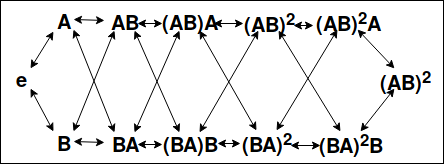
\includegraphics[scale=.6]{cayley.png}
    \caption{Cayley Graph of moves FF (=A) , RR (=B) }
    \label{fig:cayley}
\end{figure}
\vspace{10pt}
In fact this graph is not unique and is the case for a number of moves which can be applied to the cube. These moves from having an identical Cayley structure will have identical orders, thus there would exist an isomorphism between them. An example of this isomorphism could be FFRR and RRBB.


\newcommand{\ffrr}{[FFRR], F2,R2}
\newcommand{\rrbb}{[RRBB], R2,B2}
\begin{figure}[h]
\hspace{-0.5cm}
\RubikCubeSolvedWY%
\RubikRotation{\ffrr}%
\quad\SequenceBraceA{\SequenceName}{\ShowSequence{}{\Rubik}{\SequenceLong}}
\ShowCube{1.6cm}{0.5}{\DrawRubikCubeRU}%
\hspace{0.5cm}
\ShowCube{1.6cm}{0.5}{%
\DrawRubikFaceUpSide%
}
\hspace{.5cm}
\RubikCubeSolvedWY%
\RubikRotation{\rrbb}%
\quad\SequenceBraceA{\SequenceName}{\ShowSequence{}{\Rubik}{\SequenceLong}}
\ShowCube{1.6cm}{0.5}{\DrawRubikCubeRU}%
\hspace{0.5cm}
\ShowCube{1.6cm}{0.5}{%
\DrawRubikFaceUpSide%
}
\caption{Isomorphic moves FFRR, RRBB}
\label{fig:slice}
\end{figure}

As these sets of moves basically have the same result on the cube, where RRBB is is FFRR oriented 90 degrees anti-clockwise. It follows that RRBB has the exact same Cayley graph as that in figure \ref{fig:cayley}.
\paragraph*{}One more pressing problem when considering a groups structure is to find the diameter of such a Cayley graph. To find this diameter one must find the length of the longest shortest path between any two vertices on the graph. This problem applied to the Rubiks cube group becomes very difficult and for a long time was undiscovered. This algorithm is referred to as God's algorithm which will be explained in the God's Number section.

\newpage
\section{C-RAN Cubing Package (R)}

For this section on relating gods number and efficiency to actually solving the cube, it will implement the CRAN cubing package (see \ref{CRAN} for installation). From this it will
aid in the explanation about ways to solve the cube as well as showing how the mathematics behind the cube ties in with the programming.
After installing the CRAN package and using the R command to further access specific packages within CRAN , the cube functions can finally be accessed. The notation of defining the cube in terms of an array is as such:

\begin{figure}[h]
	\centering
	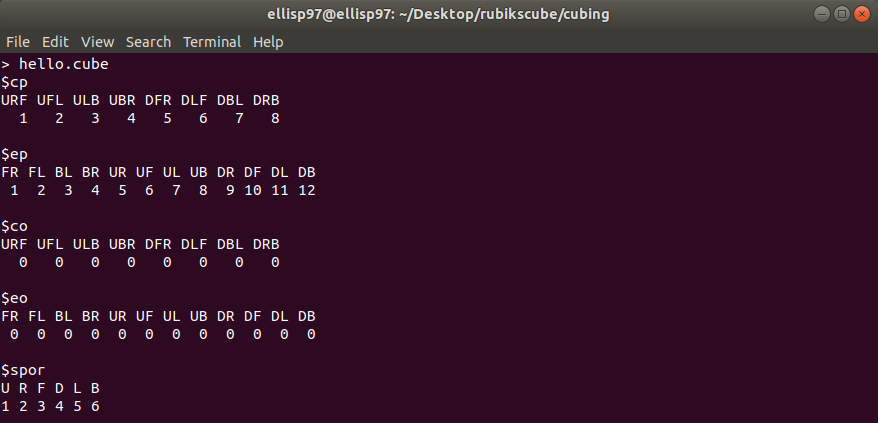
\includegraphics[scale=.5]{terminalcube.png}
	\caption{Terminal output see appendix}
\end{figure}
Entering the command hello.cube displays how the cube is stored with a similar notation to how it's labelled earlier in the project. Where \textbf{cp,ep,co,eo} stand for corner/edge permutation and orientation (where the cubies live in their cubicles).
\paragraph{}
Visual aid however is important as without this it becomes hard to see what's actually happening to the cube. This comes in 2d and 3d plots, with the commands plot(yourCube) and plot3d(yourCube) once defined (To enable the use of a 3D plot with RGL, start the RGL device in the R command) (figure \ref{fig:2d&3d}).
\afterpage{%
	\begin{figure}[p]
		\centering
		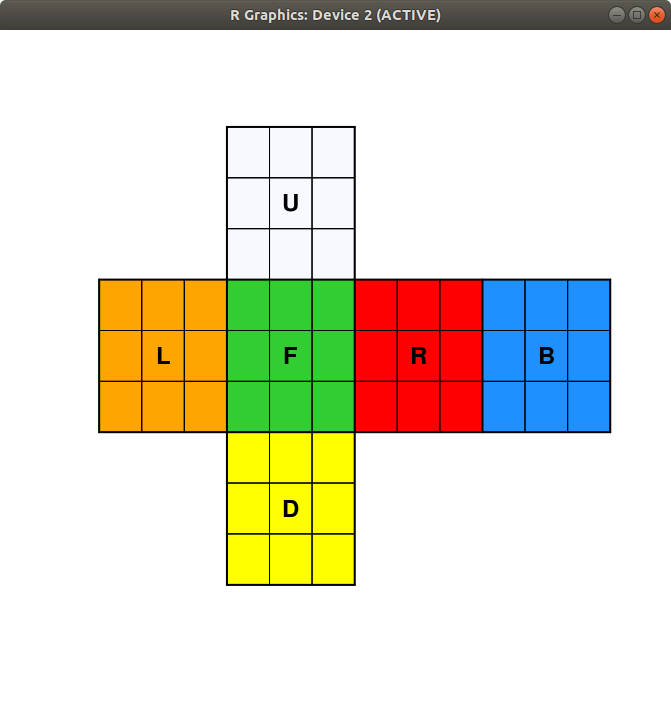
\includegraphics[scale=.4]{2dcube.png}
    	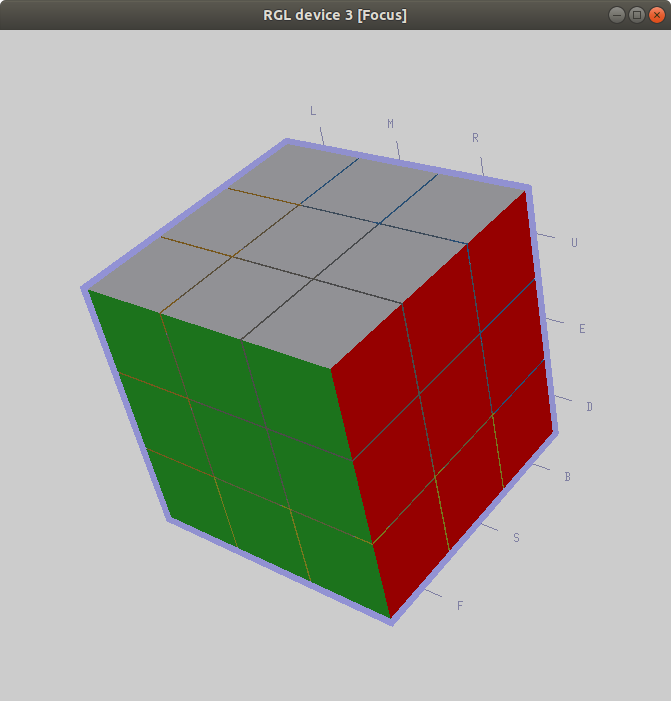
\includegraphics[scale=.4]{3dcube.png}
    	\label{fig:2d&3d}
    	\caption{2D and 3D plot of the solved cube in R}
    	\label{fig:2d&3d}
	\end{figure}
	\clearpage
}
\newpage
Using a construction like so allows the user to input any configuration of a cube into the system, whether it's valid or invalid (in terms of solvability defined previously) so long as it obeys methods of input e.g.

%\begin{lstlisting}
%>yourCube = cubieCube("UUUUUUUU RLLRRLLR BBFFFFBB DDDDDDDD LRRLLRRL FFBBBBFF")
%>plot(yourCube, numbers = TRUE)
%\end{lstlisting}


\begin{myinput}{Move seq}{i2}
\begin{itemize}
\item yourCube = cubieCube("UUUUUUUU RLLRRLLR BBFFFFBB DDDDDDDD \ \ \ LRRLLRRL FFBBBBFF")
\item plot(yourCube, numbers = TRUE)
\end{itemize}
\end{myinput}

and then can plot in usual way (including numbers = TRUE displays the cubie positions on the cube like so)(figure \ref{fig:labelled}).
\begin{figure}[h]
	\centering
	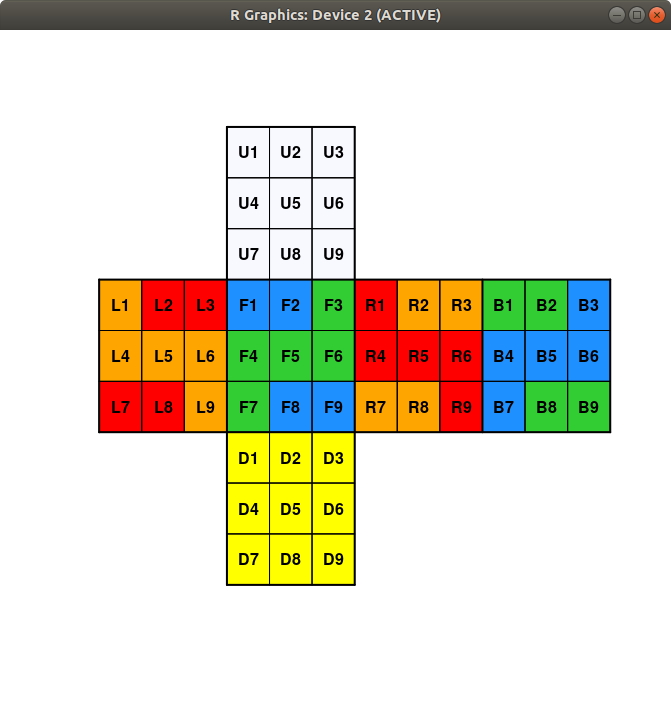
\includegraphics[scale=.5]{labelledcube.png}
	\caption{2D cube with R labelling}				    
	\label{fig:labelled}
\end{figure}
\newpage
A function which is imperative for the input of these cubes is \textbf{is.solvable}. When on input of a cube previously defined will return a boolean value depending on whether the configuration entered is correct or not.
Furthermore when a cube which has an invalid configuration has been input, 
%\begin{lstlisting}
%>is.solvable(yourCube, split = TRUE)
%
%  parity  co     eo
%  TRUE   TRUE  FALSE
%\end{lstlisting}

\begin{myinput}{Solvable Command}{i3}
\begin{itemize}
\item is.solvable(yourCube, split = TRUE)
\end{itemize}
\end{myinput}
\begin{myoutput}{Solvable Command}{o3}]
  \textbf{parity}\ \ \ \ \ \textbf{co}\ \ \ \ \ \ \textbf{eo}\\
  \ \ TRUE \ \   TRUE  \ \ FALSE
\end{myoutput}

is solvable will tell you the condition of how yourCube fails to be solvable. The items displayed above simply correspond to the fundamental theorem described earlier (theorem \ref{thm:first}), where (1) describes if \textbf{parity} is met, (2) if \textbf{co} (corner orientation) is met and (3) if \textbf{eo} (edge orientation) is met. \newline The package allows for an input of a random cube using the function randCube(). Using a combination of these functions (including is.solvable), one can construct a comparison between the ratio of solvable cubes and that statement following the equation \ref{23}.

%\begin{lstlisting}
%> sum(sapply(randCube(100, solvable = FALSE), is.solvable))
%\end{lstlisting}
\begin{myinput}{Random Cube Command}{i4}
\begin{itemize}
\item sum(sapply(randCube(100, solvable = FALSE), is.solvable))
\end{itemize}
\end{myinput}
The graph on the following page (figure \ref{fig:randomresult}) has been constructed using ten different samples of 1000 randomly generated Rubik's cubes, by equation \ref{23} the amount of cubes which should be solvable would be $1000/12 \approx 83.3$, which is the expected average.\newline 

\begin{figure}
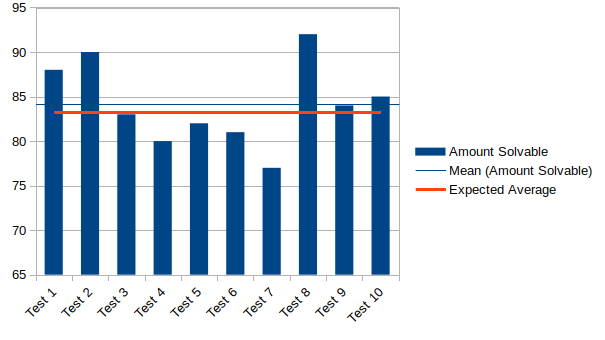
\includegraphics[scale=.8]{randomcube.png}
\caption{sample of random cubes against theorised result}
\label{fig:randomresult}
\end{figure}The actual results deviate around this mean value, with an actual mean value of 84.2 solvable cubes this is only 0.9 away from the expected means, and with more trials should converge closer to this value.\newline Using one of the following methods a user can create their own move by separating the standard moves with spaces (or even separate lines). This has uses and can be used in conjunction with the is.solvable function to see if a certain set of moves can take one configuration to the start configuration (solved).
%\begin{lstlisting}
%> yourCube <- getMovesCube(scan(what = character()))
%
%1: D2 F2 U F2 D R2 D B L' B R U L R U L2 F L' U
%20:
%19 moves read

%> mv <- scan(what = character())
%1: D2 F2 U F2 D R2 D B L' B R U L R U L2 F L' U
%20:
%19 moves read

%> result <- move(yourCube, mv)
%> is.solved(result)

%[1] TRUE
%\end{lstlisting}

\begin{myinput}{Random Cube: Method 1}{i4}
\begin{itemize}
\item yourCube $\leftarrow$ getMovesCube(scan(what = character()))
\item  D2 F2 U F2 D R2 D B L' B R U L R U L2 F L' U
\item is.solved(yourCube)
\end{itemize}
\end{myinput}

\begin{myinput}{Random Cube: Method 2}{i5}
\begin{itemize}
\item mv $\leftarrow$ scan(what = character())
\item D2 F2 U F2 D R2 D B L' B R U L R U L2 F L' U
\item result $\leftarrow$ move(yourCube, mv)
\item is.solved(result)
\end{itemize}
\end{myinput}

\begin{myoutput}{Random Cube}{o5}
19 Moves Read \\
$[1]$ TRUE
\end{myoutput}

\paragraph*{}
%\textcolor{red}{INSERT STUFF RELATING ON ANIMATION E.G. WR MOVE ANIMATE(ACUBE,MV)}
%\paragraph*{}

A question must be asked on the efficiency of this 'solver', how it works and how fast it can be done. 
The solver used in the is.solvable function is called the \textit{Kociemba Solver}. This algorithm was created by Herbert Kociemba in 1992 which is an adapted version of the Thistlethwaite algorithm often referred to as the breakthrough for cube solvers\cite{Thistlethwaite}. So to understand how efficiency works between solvers this algorithm must be considered first. Note all algorithms below use the Half-Turn Metric, this just means any one of the basic moves (quarter turn) counts as one move along with half turns such as R2, U2 etc. 

\subsection{Thistlethwaite's Algorithm}

The idea of this was to create a \textit{Divide and Conquer} style implementation, which essentially means to divide one big problem (solving the cube) into many different smaller subproblems. It uses the main concepts of group theory explained above, while utilising complex computer searches on very large lookup tables. 
The cube group $\mathcal{G}_{RC}$ is split up into the following sequence of subgroups.  

\begin{equation}
  \mathcal{G}_{RC}=\begin{cases}
    G_{0} = \text{$\opair{L,R,F,B,U,D}$}.\\
    G_{1} = \text{$\opair{L,R,F,B,U^{2},D^{2}}$}.\\
    G_{2} = \text{$\opair{L,R,F^{2},B^{2},U^{2},D^{2}}$}.\\
    G_{3} = \text{$\opair{L^{2},R^{2},F^{2},B^{2},U^{2},D^{2}}$}.\\
    G_{4} = \text{1}.
  \end{cases}
\end{equation}

This technique allows the cube to be solved in a maximum of 52 moves. Using the smaller subgroups he restricts the possible space of moves which can be made, this works by moving down the chain of $G_{0}$ to $G_{4}$ where the solved position has been found. Due to the nature of the groups $G$ they can be described as a sequence of nested subgroups. Nested subgroups allow an evaluation of the worst case scenario in the amount of moves it takes to solve using a set method. Given nested subgroups $G_1$ to $G_6$ an example can be made which explains how these subgroups help in efficiency of solving, where the below process is called \textit{The Restoration Sequence}. This moves through subgroups fixing more and more cubies each time until all cubies are in their cubicles with the correct orientation. Thus this restoration process is chracterised by the sequence of nested subgroups $G \supset G_2 \supset G_3 \supset G_4 \supset G_5 \supset G_6 $ \cite{alexander1982handbook}.
However \textit{The Restoration Sequence} works by fixing cubies at each stage, thus this can be applied to a general case. For any set of locations on the cube S, there is a subgroup G(S) which leaves the elements of S fixed. Therefore alongwith nested groups one can define a sequence of nested sets $S \supset S_2 \supset S_3 ... \supset S_n $ until the set where all cubies are fixed has been reached ($S_n$). This means for any sequence of solving the cube (not just \textit{The Restoration Sequence}) thus after step i, $G(S_i) \supset G_(S_{i+1})$ characterises that particular method. So a solving technique can be characterised by a sequence of nested subgroups but what remains to see is the converse is which is the motivation behind Thistlethwaite's Algorithm. For the algorithm in question each succesive group $G_{i+1}$ up until $G_4$ is a subgroup of the predecessor as such $G_{RC} = G_0 = G_1 = G_2 = G_3 = G_4= I$. At each stage of the algorithm a look-up table is used which shows a solution for each element in the coset space, this just means how to fix the selected cubie in the corresponding space. The table below shows how the subgroups reduce the configuration space at each stage in the Thistlewaite algorithm \cite{Thistlethwaite}.

\begin{center}
\label{:thistletab}
    \begin{tabular}{ | p{6cm} | p{4cm}| p{3cm} |}
    \hline
    Group & Configuration Number & Factor \\ \hline
    $G_{0} = \opair{L,R,F,B,U,D}$ & $4.3*10^{19}$ & 2048\\ \hline
    $G_{1} = \opair{L,R,F,B,U^{2},D^{2}}$ &  $2.1*10^{16}$ & 1,082,565\\ \hline
    $G_{2} = \opair{L,R,F^{2},B^{2},U^{2},D^{2}}$& $1.95*10^{10}$ & 29,400 \\ \hline
    $G_{3} = \opair{L^{2},R^{2},F^{2},B^{2},U^{2},D^{2}}$& $6.63*10^{5}$ & 663,552\\ \hline
    $G_{4} = I$& 1 & .\\ \hline
    \end{tabular}
\end{center}
The factor corresponds to the action of the algorithm in that stage. In stage 1 the orientation of the edges are fixed which as explained previously is the group $\mathbb{Z}_{2}^{11}$ , fixing this group is equivalent to factoring out the size of this group $2^{11} = 2048$. Similarly with stage 2 the algorithm fixes the orientations of the corners, as well as placing middle edges correctly. This corresponds to factoring out the group $\mathbb{Z}_{3}^{7}$, $3^7$  and a combinatorial argument gives the result of fixing the edge cubies in the middle to give the result $3^7 * 12!(8!*4!) = 1,082,655$. Using the lookup tables Thistlewaite was able to efficiently make use of a computer to reduce the permutations needed in a given subgroup. Thistlewaite theorised these results in a table to describe the best and worst case scenarios below.
\begin{center}
\label{:thistletab}
    \begin{tabular}{ | p{4cm}| p{1.5cm}| p{1.5cm}| p{1.5cm}| p{1.5cm}| p{2cm}|}
    \hline
    . & 1 & 2 & 3 & 4 & Total \\ \hline
    Proven Algorithm & 7 & 13 & 15 & 17 & 52\\ \hline
	Improved Proof & 7 & 13 &15 & 15 & 50\\ \hline
	Best Possible Case & 7 & 10 & 13 & 15 &45\\ \hline
    \end{tabular}
\end{center}
When published the full proof of the algorithm to reduce stage 3 to stage 4 ($G_3$ to $G_4$) was made in 17 moves by Thistlewaite. Whereas he predicted the improved case would reduce this by 2 moves, later this was correctly identified by his students. This started a somewhat trend in opening up the field of cube theory to reduce this bound. This section now relates to mentioning God's number.

\subsection{God's Number}
The number of moves it would take to solve the most difficult configuration of the cube is referred to as God's Number. If one had perfect knowledge on the Rubik's cube, would be able to solve that cube in the most efficent way using the most efficient algorithm. This is essentially just an upper bound or a worst case scenario on the maximum least number of moves from a given configuration. From the publication of Thistlewaite's proof of 52 in 1981, God's number has now been discovered from over 30 years of mathematic uncertainty to be 20 \cite{God}. \newline Previously a lower bound for God's number was thought to be 18, this is just a position which requires a minimum 18 moves to solve. However 15 years after the introduction of the cube, with the discovery of the \textit{Superflip} position this lower bound was deemed to be false.
\afterpage{
\begin{figure}
	\centering
	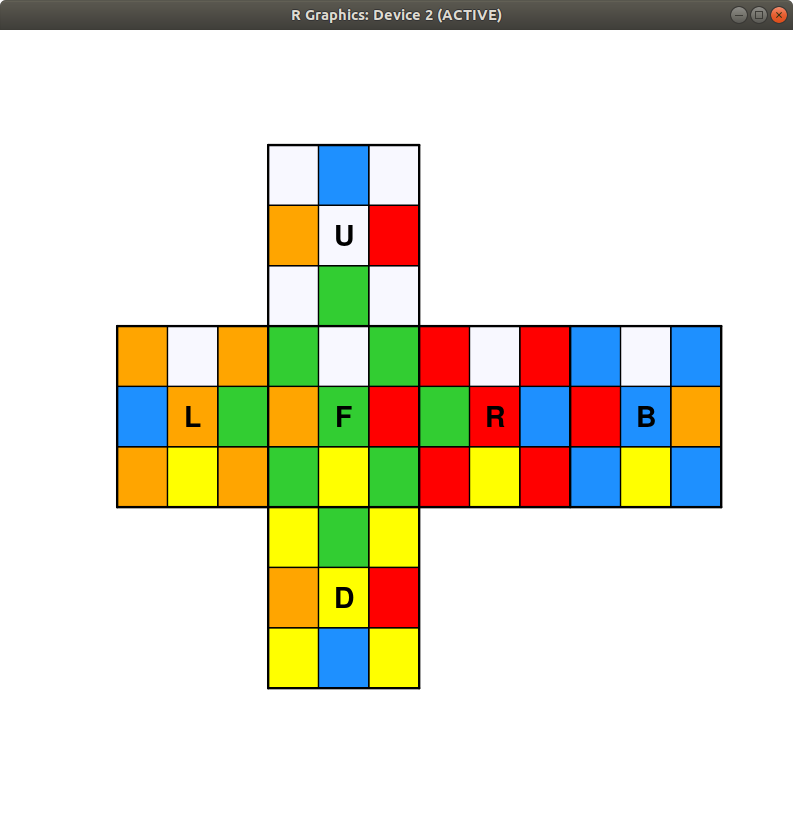
\includegraphics[scale=.37]{superflip.png}
    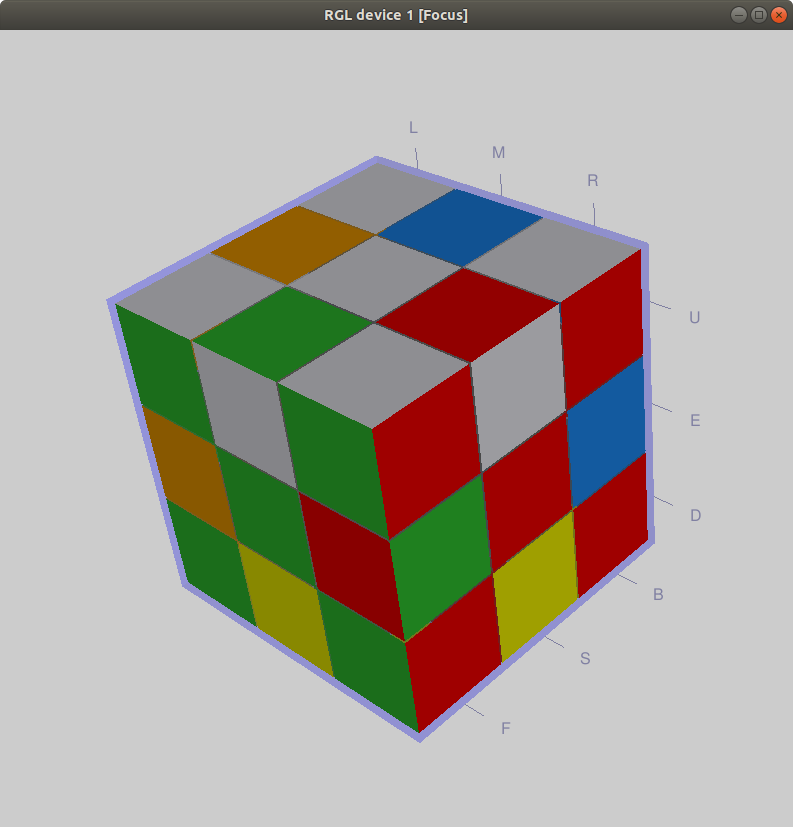
\includegraphics[scale=.37]{superflip3d.png}
    \caption{Superflip configuration in 2d and 3d}
    \label{fig:Superflipplot}
\end{figure}
\clearpage
}
This configuration is in the solved position expect that all edge pieces have incorrect orientations. A proof was made by Michael Reid in January 1995 proving that this configuration requires at least 20 moves, updating the lower bound from the previous. In fact more and more of these 20 distance configurations are being found recently where in March 2014 there were over 93 million known 20 distance positions with a total 490 million positions thought to be possible. These positions are found by analysing related cosets to positions such as the \textit{Superflip}\cite{20}. This configuration is shown on the figures following this page \ref{fig:Superflipplot}.
\paragraph*{}
What was left now was to show that this lower bound complies for all configurations , or that God's number is 20\cite{God}.
However to prove this one needed to implement a proof by exhaustion, which as previously mentioned for that time and with a sample size of $4.3 \cdot 10^{19}$ this was just computationally inefficient. This is why factoring methods such as the one in Thistlewaite's algorithm were constructed, therefore reducing the number of cases you had to check. Also a efficient way of checking if these cases could be solved was needed, motivating the explosion of these algorithms in the 30 year span.
These two optimisations were made to the full extent of the knowledge behind them, supercomputers at Google Headquarters ran this subset size of the 2.2 billion positions (reduced from the $4.3\cdot 10^{19}$) computing the result in a few weeks. Concluding that any possible configuration can be solved in a minimum of 20 moves. 
\newpage
\subsection{Computer vs God}

With optimisations and a seemingly unlimited computing power at google this still takes an infeasible amount of time when trying to solve the cube at a fast rate. So one would need to compare their efficiency with a 'God like power' who knows where every configuration can be returned to solve in a maximum number of 20 moves. As said before the algorithm used in the CRAN package uses the Kociemba Solver. This algorithm is a two phase approach. It first gets the cube in  $G_1 = \opair{U,D,R2,L2,F2,B2}$ from  $G_0$ and the second phase from $G_1$ to $G_2$ = I.  Combining both phases of Thistlewaite's algorithm to compute an efficient alternative for sub-optimal solutions on Gods algorithm. Phase 1 has a maximum length of 12, while Phase 2 has a length of 16 (previously 18 but last 2 can be avoided), thus the whole bound of Kociemba's Algorithm is 28. This stood for a number of years as the global optimum before the proof for God's number as 20 in 2010\cite{Rokicki2013TheDO}. The algorithm uses backtracking in both phases to lower this bound to attempt to retrieve an optimal solution. It does this by implementing the following algorithms:

\begin{lstlisting}
function KociembaAlg(position)
	loop depth from 0 to maxLength:
		Phase1Search(position,depth)
	end loop
end function
\end{lstlisting}
\begin{lstlisting}
function Phase1Search(position,depth)
	if depth = 0 then:
		if last move was a quarter turn of [R,L,F,B] and subgoal reached then:
			Phase2Search(position)
		end if
	else if depth > 0 then:
		if prune1[position] <= depth then:
			loop through all moves M:
				Phase1Search(M applied to position, depth -1)
			end loop
		end if
	end if
end function
\end{lstlisting}
\begin{lstlisting}
function Phase2Search(position,depth)
	loop depth from 0 to maxLength - currentDepth
		if depth = 0 then:
			if cube solved:
				"solution found"
				maxLength = currentDepth - 1
			end if
		else if depth > 0 then:
			if prune2[position] <= depth then:
				loop through all moves M:
					Phase2Search(M applied to position, depth -1)
				end loop
			end if
		end if
	end loop
end function
\end{lstlisting}
This format of the Kociemba Algorithm is also in pseudo code to make ease of understanding for the reader, thus line by line it just be fairly trivial to understand what it's doing. Although it also uses new aspects uncovered previously, for instance in Phase1Search it looks in the pruning table and makes a comparison to the depth. The pruning table will provide a lower bound for a given position on the number of moves needed to solve. This may seem more powerful at first, as this implies full efficiency, hence Gods number. However this is not the case as a pruning table does not change for each configuration of the cube, and instead represents a set of similar configurations as an index. So God's algorithm is essentially identical however the full position is stored, as opposed to part of the position to index the pruning tables like in Kociemba. The full explanation of the algorithm can be found on Kociemba's personal website \cite{kocweb}.\newline A comparison could be made to test the efficiency between the two by graphing out some results. However as computing power of google's computers is hard to come by, also alongwith a sensible time constraint this makes a comparison between the two difficult. From Tomas Rokiki paper the optimised version of Kociemba's Algorithm can calculate 3900 20-length (max-length) solutions. The time to solve all positions using this method is around 3.7 million CPU years \cite{Rokicki2013TheDO}. However slow it is still much faster than several billion years for a perfect solution for each configuration. The below table shows this efficiency argument, additionally combining the rate for solving a coset at a time. The first row displays positions done per second between a perfect algorithm and the one in question, while the second displays cosets at a time.

\begin{center}
\label{:thistletab}
    \begin{tabular}{ |p{5cm}| p{4cm}| p{4cm}|}
    \hline
    . & Optimal Solution & Near Optimal \\ \hline
    Individual Position & 2 & 3900\\ \hline
	Cosets of the Cube Group & $2*10^6$  & $10^9$\\ \hline
    \end{tabular}
\end{center}

\newpage
\section{Pocket Cube}

\begin{figure}[h]
\centering
  \TwoCubeSolved%
  \TwoRotation{R}
  \TwoRotation{L}
  \ShowCube{4cm}{1}{\DrawTwoCubeRU}
\end{figure}

There have been a lot of variants made since the production of the original 3x3x3 Rubik's cube in 1974. These include 4 by 4, 5 by 5's, tetrahedron and triangular based cubes and so on. The majority of these cubes aim to heighten the difficulty of the original puzzle, where more complex moves and algorithms would be needed. However describing the original 3 by 3 cube already implements a high brute force cost on computational efficiency. Here the 2 by 2 cube is introduced to show the comparison between the two, and how the group size grows exponentially. The following will explore the basic structure of the pocket cube along with analysing Daniel Bump and Daniel Auerbachs paper on the miniature Rubik's cube and it's two generator group. This extends from Singmasters introduction of the two-generator group and the fascination behind it.
\paragraph*{}
Again the 2 by 2 cube has the exact same set of basic moves M = $\{L,R,U,D,F,B\}$. However this time the group structure will differ a lot because there are no such edge cubies. It is made up of just 8 cubes which can act similarly to corner cubies using the group already defined ($\mathbb{Z}_{3}^{7}$). The proof of the pocket cube being a group is identical to that of the 3 by 3 cube.
For the basic moves of the pocket cube, similar to the 3 by 3, there is disjoint cycle notation which describe the action of performing the respective move on the cube. 
\begin{align*}
U&=(5,13,21,17)(6,14,22,18)(1,2,4,3)\\
R&=(6,22,3,10)(8,4,21,12)(17,18,20,19)\\
F&=(5,6,7,8)(3,17,10,16)(14,4,19,9)\\
D&=(7,19,23,15)(8,20,24,16)(9,10,11,12)\\
L&=(13,14,16,15)(5,9,24,1)(7,11,22,3)\\
B&= (21,22,24,23)(2,13,11,20)(1,15,12,18)
\end{align*}
These cycles are based on the following labelling of the cube(figure \ref{fig:2labelling}), similar to the 3 by 3 but there are now only 4 cubies to label not 9 on each face. The previous notation on conservation of parity for corners in theorem \ref{thm:first}(2) can be applied to this cube in defining the structure. In a similar way to showing the 3 by 3 is a semi-direct product the 2 by 2 can be, with a far more simpler evaluation of 
\begin{equation}
G = \mathbb{Z}^{7}_{3} \rtimes S_8
\end{equation}
This order of this group can be calculated as $(3^7)\cdot 8!$ = 88,179,840. This number also includes all the non valid positions of the pocket cube, so it doesn't reflect the true legal 2 by 2 group thus to find the legal value one must go about considering reducing by the false cases. However in the cube group as as it is by an even number n (n by n by n) there are no fixed cubies the total order cannot be factored in the same way as the 3 by 3. As there are only corner cubies, and those which differ in orientation are equivalent, there are $3\cdot 8=24$ ways to orient in the orbit space. This gives a new order of 88,179,840/24 = 3,674,160.
The table below describes the distance from the solved configuration, showing these different positions and the maximum number of half or quarter turns needed to get back.

\begin{center}
\label{:thistletab}
    \begin{tabular}{ | p{3cm} | p{6cm}| p{6cm} |}
    \hline
    Number of Moves, N  & Positions that require N moves (Half or Quarter) & Positions that require N moves (Quarter only) \\ \hline
     0 & 1 & 1\\ \hline
     1 & 9 & 6\\ \hline
     2 & 54 & 27\\ \hline
     3 & 321 & 120\\ \hline
     4 & 1847 & 534\\ \hline
     5 & 9992 & 2256\\ \hline
     6 & 50136 & 8969\\ \hline
     7 & 227536 & 33058\\ \hline
     8 & 870072 & 114149\\ \hline
     9 & 1887748 & 360508\\ \hline
     10 & 623800 & 930588\\ \hline
     11 & 2644 & 5341350852\\ \hline
     12 & 0 & 782539\\ \hline
     13 & 0 & 90280\\ \hline
     14 & 0 & 276\\ \hline
    \end{tabular}
\end{center}

This is a large reduction on the 3 by 3 group but still comes with quite a large set, especially considering computational costs. This gives motivation for introducing the two generator group for the pocket cube which dramatically improves these costs, where this group has order 29160 \cite{bandelow2012inside}. Thus for the pocket cube in a half turn metrics God's number is 11.

\begin{figure}[h]
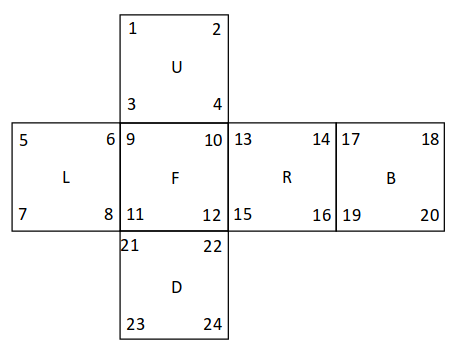
\includegraphics[scale=.5]{2by2.png}
\caption{Labelling of the Pocket Cube}
\label{fig:2labelling}
\end{figure}\paragraph{}
\newpage
\subsection{Two Generating Group}

However for this cube the minimal generating subgroup can be generated by just two moves as opposed to 5. So the two generating subgroup G is denoted as $G = \langle R, U\rangle$. Also the non valid configurations must be considered, so one will need to consider the valid group of the pocket cube. When applying a move to the pocket cube, one can see similar to that of the ($\mathbb{Z}_{3}^{7}$) subgroup thus the last cubie will be determined automatically (as in the 3 by 3). While in this version of the cube any the orientation group can be defined as the subgroup of G, say K. This which can also be thought of as the basic move operations that dont't change the position of any other 6 cubies \cite{bump2006unravelling}. As the orientation subgroup K only describes the change of orientations of cubies, it does not depend on order operations are performed. Thus the subgroup is abelian, but trivially by inspecting moves the pocket cubes group must not be. It follows from the definition that K is a normal subgroup of G as gK = Kg,or equivalently for $g \in G$ an operation, $gKg^{-1} = K$. To get a bound on the pocket cube group, one must first get a bound on the orientation subgroup to which it's defined by. There are 3 possible orientations for each of the 6 cubies, and following from  the fundamental theorem for cube theory (note this still applies for the pocket cube as all individual cubies here are essentially acting as corner cubies) (theorem \ref{thm:first}(2)) these orientations must equal 0 (mod 3). Again note that 6 cubies are considered as the original group is a 2-generated group by the two moves R,U which by inspection only effect 6 cubies on the pocket cube. Thus there is a free choice for 5 of the 6 corners which are movable, while the remaining one is determined automatically by construction. This means that the bound for the subgroup K must be $|K| \leq 3^5$. To show $|K| \leq 3^5$ there just needs an example given to show there is a move which generates the group from the elements of the two generator such that it equals 0 (mod 3). Such a move is:
\begin{equation}
RUR^{-1}URU^{2}R^{-1}U^{2} \in K
\end{equation}

\newcommand{\changecorner}{[Orient 3 Corner],R,U,Rp,U,R,U2,Rp,U2}%
\newcommand{\changecornerarrow}{$\quad\overrightarrow{\strut\textsc{Orienting the corner}}\quad$}

\begin{figure}[h]
\centering
  \TwoCubeSolved%
  \ShowCube{4cm}{1}{\DrawTwoCubeRU}\changecornerarrow
  \TwoRotation{\changecorner}
  \ShowCube{4cm}{1}{\DrawTwoCubeRU}
  \caption{Move showing the corners beingpermuted}
\end{figure}
Thus the bound on the subgroup is $K = 3^5$.\newline H described these orientations of the 6 cubies in their cubicles. There must be a group such that it describes permutations which affect the locations of the 6 pieces.
It's useful here to introduce the notion of a projective general linear group. 

\subsection*{Projective General Linear Group (PGL)}
The projective general linear group denoted PGL(n,k) of order n over k where $n \in \mathbb{N}$, k a field is defined such that:
\begin{itemize}
\item It's the group of automorphisms of projective space of dimension n-1, that arise from linear automorphisms of the vector space of dimension n
\item It's the quotient of GL(n,k) by it's center C, the scalar matrices of the identity
\end{itemize} 

The elements can be projected onto $\mathbb{P}^{1}(\mathbb{F}_5)$ this just describes labelling of points of the line $\mathbb{P}$ over a field with 5 elements. One can individually reference cubie locations here, considering the 3 by 3 rubiks cube there would be far too many elements to talk about projective line mapping. The quotient group $G/K$ fits this definition of the group of permutations on $\mathbb{P}^{1}(\mathbb{F}_5)$ which exclude orientation. Using this definition one can accurately reference the group e.g. instead of calling it a subgroup of $S_6$ and deal with non valid permutations. So from the definition above, the group of permutations is PGL(2,$\mathbb{F}_5$) acting on elements $\mathbb{P}^{1}(\mathbb{F}_5)$ by fractional linear  transformations. From there one can tell the generalised linear group GL(2,$\mathbb{F}_5$) below which describes all the invertible matrices.
\begin{equation}
\begin{pmatrix} a & b \\ c & d \end{pmatrix} : x \mapsto \frac{ax + b}{cx + d},\ \ \ \ \ x \in \mathbb{P}^{1}(\mathbb{F}_5)
\end{equation}

The projective line here is actually the projective extended real line due to working in real numbers. It extends the number line to which the elements are mapped onto by a infinity point $\infty$. This infinite point describes the point to which both ends of the real number line (sequence) meet, the limit of the sequence. One can also think about any such parallel lines on a visual plane that despite no intersection $\infty$ can be used to categorise such lines. Taking this information into the equation above, $x \in \mathbb{P}^{1}(\mathbb{F}_5)$ simply means $x \in \mathbb{F}_5 \cup \infty$. Thus for $x = \infty$, $\frac{ax + b}{cx + d} = \frac{a}{c}$ and for $x = 0$, $\frac{ax + b}{cx + d} = \infty$. As from the definition the center C of the generalised group GL(2,$\mathbb{F}_5$) consists of the scalar matrices on the identity, which is just the kernel of the generalised group. An action of the group G is actually just an action on GL(2,$\mathbb{F}_5$)/C = PGL(2,$\mathbb{F}_5$), giving the desired action on the group of cubie locations. This can be shown formally below:
\newpage
\begin{prop}[Singmaster]{Singmaster}
The permutation group acting on $\mathbb{P}^{1}(\mathbb{F}_5)$ is G/K = PGL(2,$\mathbb{F}_5$)
\end{prop}

\begin{prf}{prf:Singmaster}
To see this one needs to check that the generators of the quotient G/K (and thus the moves) are contained in PGL(2,$\mathbb{F}_5$). As the group is two generated from U,R , one just needs to show U,UR (or a combination of such) $\in$ PGL(2,$\mathbb{F}_5$). With the labelling in \ref{fig:2labelling}, U generates the cycle (10,9,1,$\infty$) and UR generates (10,9,1,16,12). Now look at their fractional transformations by comparing the signs of the respective cubies.

\paragraph{These U and UR moves on the pocket cube can be seen on the page following \ref{fig:UR}}
\paragraph*{}
\begin{equation}
U = \begin{pmatrix} 0 & 1 \\ 2 & 1\end{pmatrix} \in \text{PGL}(2,\mathbb{F}_5) \ \ \ \ \ \ \ \ \ \ \ \ \ \ \ \ \ \ \ \ 
UR = \begin{pmatrix} 1 & 1 \\ 0 & 1\end{pmatrix}\in \text{PGL}(2,\mathbb{F}_5)
\end{equation}
In particular this linear transform for both of these can be examined. For U there is 
\begin{equation*}
x \mapsto \frac{1}{2x + 1}
\end{equation*}
, and for UR there is 
\begin{equation*}
x \mapsto \frac{x+1}{1}
\end{equation*}
such that using these transforms one can show that these moves are in fact $\in$ PGL(2,$\mathbb{F}_5$). This is done by checking each element in the field $\mathbb{F}_5$ (congruent mod 5) under the remains in the permutation group.
\begin{alignat*}{2}
& \begin{aligned}
0 &\mapsto \frac{1}{2*0 + 1} = \frac{1}{1} = 1\\
1 &\mapsto \frac{1}{2*1 + 1} = \frac{1}{3} = 3^{-1} \equiv 2\\
2 &\mapsto \frac{1}{2*2 + 1} = \frac{1}{5} \equiv \frac{1}{0} = \infty\\
3 &\mapsto \frac{1}{2*3 + 1} = \frac{1}{7} \equiv \frac{1}{2} = 2^{-1} = 3\\
4 &\mapsto \frac{1}{2*4 + 1} = \frac{1}{9} \equiv \frac{1}{4} = 4
\end{aligned}
& \hskip 6em &
\begin{aligned}
0 &\mapsto \frac{0 + 1}{1} = \frac{1}{1} = 1\\
1 &\mapsto \frac{1 + 1}{1} = \frac{2}{1} = 2\\
2 &\mapsto \frac{2 + 1}{1} = \frac{3}{1} = 3\\
3 &\mapsto \frac{3 + 1}{1} = \frac{4}{1} = 4\\
4 &\mapsto \frac{4 + 1}{1} = \frac{5}{1} \equiv \frac{0}{1} = 0
\end{aligned}
\end{alignat*}
Where on the left there's the transformation for U, and the UR for the right. Note $\infty \mapsto 0$ in U and $\infty \mapsto \infty$ in UR. Thus all elements have been checked and $G/K \subset$ PGL$(2,\mathbb{F}_5)$. Combined with the fact these two elements generate PGL$(2,\mathbb{F}_5)$ gives the desired result. 
\end{prf}

\begin{figure}[h]
\centering
  \TwoCubeSolved%
  \TwoRotation{U}
  \Rubik{U}
  \ShowCube{4cm}{1}{\DrawTwoCubeRU}
  \TwoCubeSolved%
  \hspace{2cm}
  \Rubik{U}\Rubik{R}
  \TwoRotation{U}\TwoRotation{R}
  \ShowCube{4cm}{1}{\DrawTwoCubeRU}
  \caption{U and UR move on the pocket cube}
  \label{fig:UR}
\end{figure}

The moves which generate the group U,R only change the positions of the 6 cubies, but the last one is determined. Following this it can be shown there is an isomorphism between this and the symmetric group $S_5$. Firstly though it is needed to show that this quotient has identical order to the symmetric group to construct such a map \cite{bandelow2012inside}.

\begin{prop}[Symmetric Size Equality]{prop:5fac}
The quotient group if of size $|G/H|$ = 5!
\end{prop}
\begin{prf}{prf:5fac}
Proving this is identical to showing that the size of PGL$(2,\mathbb{F}_5)$ = 5!. From the definition the projective general linear group is the quotient of the general linear group GL(2,$\mathbb{F}_5$) over it's centre. So to determine the size of PGL$(2,\mathbb{F}_5)$, firstly one must find the size of the GL(2,$\mathbb{F}_5$). All zero determinant scalar matrices are contained in the centre of the quotient , so GL(2,$\mathbb{F}_5$) is all these non zero  matrices in the field. For the matrices of the form $\begin{pmatrix}a & b \\ c & d\end{pmatrix}$, there are 5 choices for each element, meaning there are $5^{4}$ = 625 possible elements. However these include the zero  matrices to which are contained in the centre. So to get the actual number, the centre can be calculated and then quotioned out. 

There is a zero matrix when the determinant of the matrix is zero, or for the above case when $a\cdot d$ - $b\cdot c$ = 0. Thus the following cases of zero determinant matrices must be considered. 
\begin{itemize}
\item $a \neq, d \neq 0, b \neq 0$. Here there are 4 choices in the field for a and d and b and c is fixed as a field contains no zero divisors. So if $b\cdot c$ = 0 with $b \neq 0$, there is only one option for c. So there are $4\cdot4\cdot4\cdot1$ = 64 choices here.
\item  $a \neq 0, d = 0, b \neq 0$. Here there are 4 choices for a and b, d is fixed by the case. So for a 0 determinant here $b\cdot c$ must also equal 0 thus fixing c to one choice. So there are $4\cdot 1\cdot 4\cdot 1$ = 16 choices.
\item $a = 0, d \neq 0, b \neq 0$. Again this is similar to the above case, so 16 more choices.
\item $a \neq 0, d = 0, b = 0$. Again 4 choices for a, b and d are fixed by the specific case. Thus c can be any choice of 5 as determinant is already 0. So there are $4\cdot 1\cdot 1\cdot 5$ = 20 choices.
\item  $a = 0, d \neq 0, b = 0$. This is identical to above case, so 20 more choices.
\item $a = 0, d = 0$. For the determinant to be 0 in this case it just needs b or c to be 0. So there are 5 choices for b when c is 0, and vice versa. The case where b and c are 0 is counted twice so needs to be decremented from the toal thus $2\cdot (1\cdot 1\cdot 1\cdot 5)$ - 1 = 9 choices. 
\end{itemize}
So totalling the non zero determinant possibilities gives 64+16+16+20+20+9 = 145 possible elements contained in the centre. Thus GL(2,$\mathbb{F}_5$) contains (625-125) 480 elements. So for the size of PGL(2,$\mathbb{F}_5)$ we quotient out this value with the size of the centre C , $480/|C|$, giving PGL(2,$\mathbb{F}_5)$ = 480/4 = 120 (=5!).
\end{prf}

Next move on to show the isomorphism as described earlier:

\begin{prop}[Symmetric Isomorphism]{prop:symiso}
The quotient group is isomorphic to the 5-symmetric group, G/K $\cong S_5$
\end{prop}
\begin{prf}{prf:iso}
To show G/K or PGL(2,$\mathbb{F}_5)$ is isomorphic to the symmetric group of 5 elements one needs to consider the 5 Sylow groups. For a p prime , the highest power $p^{k}$ which divides the order of the group means there exists a subgroup of G, of order $p^{k}$ called a p-Sylow subgroup. Taking the group G as the symmetric group $S_5$ the 5-Sylow subgroup can be labelled in the following way: 
\begin{alignat*}{2}
& \begin{aligned}
\infty &= \langle (1,2,3,4,5) \rangle\\
1 &= \langle (1,2,3,5,4) \rangle \\
2 &= \langle (1,2,4,5,3) \rangle \\
\end{aligned} 
& \hskip 6em &
\begin{aligned}
3 &= \langle (1,2,5,4,3) \rangle \\
4 &= \langle (1,2,5,3,4) \rangle \\
5 &= \langle (1,2,4,3,5) \rangle
\end{aligned}
\end{alignat*}
%REFERENCE GENERATOR THING IF HAVENT ALRWEAY%

Conjugating these above subgroups will describe how $S_5$ acts on the permutation group $\mathbb{P}^{1}(\mathbb{F}_5)$. The claim to show the isomorphism is that the group of permutations as a result of conjugacy is in fact PGL(2,$\mathbb{F}_5)$. The action of conjugacy is described below:

\subsubsection{Conjugate Subgroup}
For a subgroup H with elements $k_{i}$ and a fixed element x $\in$ G,where x $\not\in$ K. The transformation $xk_{i}x^{-1}$ for (i=1,2,...) generates the conjugate subgroup. 
\paragraph*{}
Where in this case taking K as a Sylow subgroup $\in \{\infty,0,1,2,3,4\}$ and x a fixed element of an alternate cycle the operation can proceed. To see the group obtained is PGL(2,$\mathbb{F}_5)$ one must check the generators of $S_5$ induces linear fractional transformation as in the proof of the previous proposition \ref{Singmaster}. Taking conjugation on the subgroup $\infty = \langle(12345) \rangle$ gives the following:
\begin{align*}
(12345)(12345)(12345)^{-1} &= (12345) :\infty \mapsto \infty \\
(12345)(12354)(12345)^{-1} &= (15234) :0 \mapsto 1\\
(12345)(12453)(12345)^{-1} &= (14235) :1 \mapsto 2\\
(12345)(12543)(12345)^{-1} &= (12534) :2 \mapsto 3\\
(12345)(12534)(12345)^{-1} &= (14523) :3 \mapsto 4\\
(12345)(12435)(12345)^{-1} &= (13425) :4 \mapsto 0
\end{align*}
Where the fixed element x has been chosen from the group $S_5$'s Sylow subgroups. This conjugation creates the transformation which fixes $\infty$ and permutes the cycle (01234). Thus this linear transformation is just $x \mapsto x + 1$ (where $x \neq\infty$). This transformation corresponds to the matrix $\begin{pmatrix} 1 & 1 \\ 0 & 1\end{pmatrix} \in$ GL(2,$\mathbb{F}_{5})$. Secondly consider another conjugation which produces a similar result namely the conjugation on the transposition (45). This is shown  below:
\begin{align*}
(45)(12345)(45) &= (12354) :\infty \mapsto 0 \\
(45)(12354)(45) &= (12345) :0 \mapsto \infty\\
(45)(12453)(45) &= (12543) :1 \mapsto 2\\
(45)(12543)(45) &= (12453) :2 \mapsto 1\\
(45)(12534)(45) &= (12435) :3 \mapsto 4\\
(45)(12435)(45) &= (12534) :4 \mapsto 3
\end{align*}
As a transposition, cycle of 2 elements, is conjugated by it's inverse which in this case is identical to itself, $(45)^{-1}$ = (45). To see it's linear transform inspect the maps on the field (mod 5), similarly as in the proof of \ref{Singmaster} this can be shown like so:
\begin{alignat*}{2}
& \begin{aligned}
0 &\mapsto \frac{2}{0} = \infty\\
2 &\mapsto \frac{2}{2} = 1 \\
4 &\mapsto \frac{2}{4} = 2\cdot 4^{-1} \equiv 2\cdot 4 \equiv 3
\end{aligned}
& \hskip 6em &
\begin{aligned}
1 &\mapsto \frac{2}{1} = \frac{2}{2} = 2\\
3 &\mapsto \frac{2}{3} = 2\cdot 3^{-1} \equiv 2\cdot 2 = 4
\end{aligned}
\end{alignat*}
By inspection the map is $x \mapsto \frac{2}{x}$ which is verified above, permuting like so $0 \leftrightarrow \infty, 1 \leftrightarrow 2, 3 \leftrightarrow 4$. With the corresponding matrix $\begin{pmatrix} 0 & 2 \\ 1 & 0\end{pmatrix} \in $GL($2,\mathbb{F}_{5})$. It can be seen that these cycles (12345) and (45) generate $S_5 (= \langle (45),(12345) \rangle$). This is done by comparing all elements in $S_5$, which are products of transpositions, with any transpositions produced by the generating set  $\langle (45),(12345) \rangle$. This can be done fairly easier when considering the size of the groups considered. So every permutation of the 5-Sylow subgroup from the labelling above is contained PGL(2,$\mathbb{F}_5$), thus using the above one can construct a homomorphism $\phi : S_5 \rightarrow $PGL(2,$\mathbb{F}_5)$. This just describes the actions already described sending transpositions in the symmetric group to the projective line group. As both groups have identical order of 5! = 120, the homomorphism maps between equal order groups thus there is an isomorphism giving the required statement G/K $\cong S_5$. 
\end{prf}

Now with the above propositions and definitions it is enough to formally define the pocket cube. The conditions for semi-direct product are that K is a normal subgroup of G (which has already been shown in showing the bound of K), and also that G is the product of these subgroups such that G = KH where $K \cup H$ = e , and H is the subgroup permuting the 6 cubies in question. This follows as K strictly changes orientation and does not permute the cubes. Thus can be formalised G = $K \rtimes H$ for the two generator group.

\subsection{Devil's Algorithm}

As one application on the pocket cube the 'Devil's Number' is considered. Think of the devil as a somewhat opposite to God, where due to a manageable sized group in the pocket cube a solution can be found, which is not necessarily that efficient. In particular this algorithm is the set of moves which can be applied a said amount of times which will always return the solved configuration of the cube. Where this said amount of times is the Devil's Number. So one can restrict the pocket cube group to the half turn metric, by only allowing moves R2, U2, B2 etc.
This makes the over 3 million size of the quarter turn metric much more managable. It turns out for this restricted group the Devil's Number is 7\cite{Devil}.
The Devil's algorithm move sequence for this group is RURURBR giving an updated table below.

\begin{center}
\label{:thistletab}
    \begin{tabular}{ | p{6cm} | p{6cm}|}
    \hline
    Number of Moves, N  & Number of Possible Configurations \\ \hline
     0 & 1\\ \hline
     1 & 3\\ \hline
     2 & 6\\ \hline
     3 & 9\\ \hline
     4 & 5\\ \hline
     Total & 24\\ \hline
    \end{tabular}
\end{center}

Thus using this group, someone with no knowledge, or even eyes, on the cube will stand a good chance of solving by using the algorithm at any specific point. This number can be verified from the Cayley Graph as there is only a total of 24 configurations, which makes drawing the graph (figure \ref{fig:doubleturn})\cite{Devil} possible. (Note any quarter turn will break this group from it's orbit).

\begin{figure}[h]
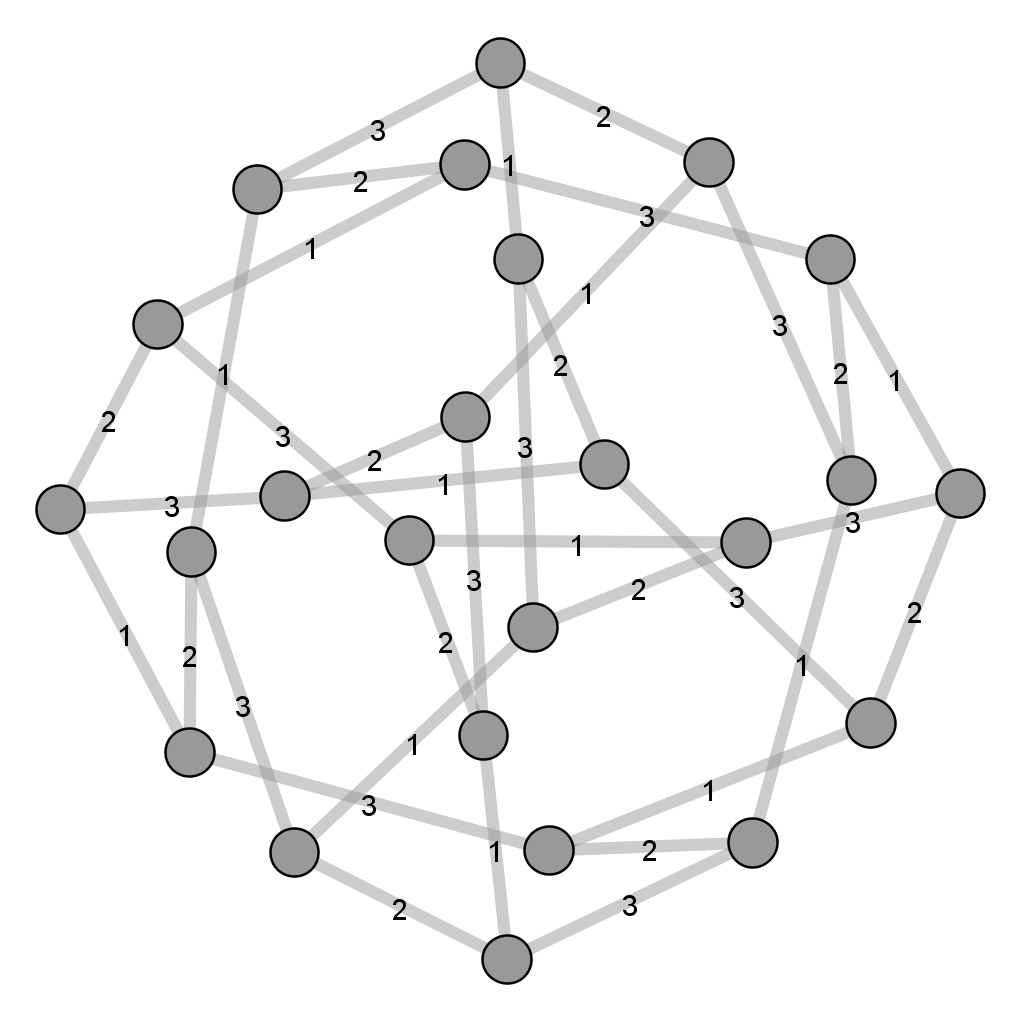
\includegraphics[scale=.15]{DoubleTurn.png}
\caption{Cayley Graph of the restricted Pocket Cube}
\label{fig:doubleturn}
\end{figure}

Just as an indicator on how restricting these groups are important to efficiency costs consider the unrestricted groups. Devils number for the 2 by 2 is between 102060 and 2886840 and for the 3 by 3 is between 4,326,986,725,785,600 and 43,251,683,287,486,463,996.
%Where earlier saw the 3 by 3 cube had a subgroup for the orientation group , one which changed corner pieces, it seems isomorphic ORNOT

\newpage

\section{Conclusion}

This project has analysed the Rubik's cube in depth by relating complex group structure to the composition of the cube. The theorems and lemmas within group theory have allowed problems to be solved on the mysteries that lie within the cube. The fascination behind this puzzle has led discoveries in recent years from the evaluation of God's number to the construction of real time efficiency solvers. This paper uses the aid of many valuable resources in particular Singmasters "Notes on Rubik's Magic Cube", which for a first time solver is extremely useful. The conclusion of the most efficient algorithms with the bounds has been found for both the 2 by 2 and the 3 by 3, as 11 and 20 moves (half turn metric) respectively. Where todays technology has reached the point to evaluate a 43 trillion size group, researches hope to move on to the 4 by 4 cube. Which truly shows you can't have a group too big.

\paragraph{}
\paragraph{}

\subsubsection{CRAN}
\label{CRAN}
The CRAN-R package works on MacOS, Windows and Linux versions. Please see the official CRAN page for instructions on installation (https://cran.r-project.org/) . From there install the 'cubing' (https://cran.r-project.org/web/packages/cubing/index.html) and 'rgl' libraries to enable functionality.
%include something before on order of some moves

\newpage

%\bibliographystyle{apacite}
\printbibliography

\end{document}

